\documentclass[a4paper, 12pt]{article} % Artikel-Klasse

%---------------------------------------------------------
% Encoding, language, quotes
%---------------------------------------------------------
\usepackage[utf8]{inputenc}
\usepackage[ngerman]{babel}       % Deutsche Sprache und Silbentrennung
\usepackage{csquotes}             % Für korrekte Anführungszeichen
\usepackage{listings}
\usepackage{xcolor}

%---------------------------------------------------------
% Graphics & PDF
%---------------------------------------------------------
\usepackage{graphicx}
\usepackage{pdfpages}             % Einbinden von PDF-Seiten
\usepackage{caption}              % Verbesserte Bildunterschriften
\usepackage{subcaption}

% Customize settings
% Customize settings for a more compact style
\lstset{
    language=Java,                 % Specify Java language for syntax highlighting
    basicstyle=\ttfamily\small,    % Use smaller monospaced font for code
    keywordstyle=\color{blue},     % Style for keywords
    commentstyle=\color{gray},     % Style for comments
    stringstyle=\color{red},       % Style for strings
    numbers=none,                  % No line numbers
    breaklines=true,               % Break long lines
    frame=none,                    % No frame around the code
    xleftmargin=0pt,               % Remove left margin
    xrightmargin=0pt,              % Remove right margin
    aboveskip=5pt,                 % Reduce space above the code block
    belowskip=5pt                  % Reduce space below the code block
}

%---------------------------------------------------------
% Math, units, spacing, etc.
%---------------------------------------------------------
\usepackage{siunitx}
\usepackage{setspace}
\usepackage{textgreek}

% Add float package for "H" float option
\usepackage{float}

%---------------------------------------------------------
% Other packages
%---------------------------------------------------------
\usepackage{ifthen}
\usepackage{acronym}
\PassOptionsToPackage{hyphens}{url} % URLs in Hyperlinks umbrechen
\usepackage[breaklinks=true]{hyperref} 
\usepackage{array}                % Bessere Tabellenformatierung
\usepackage{enumitem}             % Kontrolle über Listen-Layouts
\usepackage{nomencl}
\usepackage{scrlayer-scrpage}     % Header und Footer

% Adjust header and footer heights
\setlength{\headheight}{14.5pt}
\setlength{\footheight}{34.16666pt}

%---------------------------------------------------------
% Bibliography (biblatex mit Biber)
%---------------------------------------------------------
\usepackage[backend=biber, style=ieee]{biblatex}  
\addbibresource{literatur.bib}  

%---------------------------------------------------------
% Platzhalter
%---------------------------------------------------------
\newcommand{\titel}{Verbesserung eines Bluetooth-basierten Warnsystems für den Straßenverkehr durch Datenlogging und innovative Visualisierungstechniken}
\newcommand{\untertitel}{}
\newcommand{\arbeit}{Studienarbeit T3200}
\newcommand{\studiengang}{Elektrotechnik}
\newcommand{\studienrichtung}{Fahrzeugelektronik}
\newcommand{\autor}{Luka Tadic}
\newcommand{\abgabe}{14.07.2025}
\newcommand{\bearbeitungszeitraum}{07.04.2025 - 14.07.2025}
\newcommand{\matrikelnr}{5726700}
\newcommand{\kurs}{TFE22-1}
\newcommand{\firma}{}
\newcommand{\betreuerfirma}{Prof. Dr. Ing. Tobias Frank}
\newcommand{\gutachterdhbw}{Prof. Dr. Ing. Tobias Frank}
\newcommand{\jahr}{2025}

%---------------------------------------------------------
% Header und Footer mit Linien
%---------------------------------------------------------
\clearpairofpagestyles         % Standard-Stile löschen

% Header with consistent logo placement and line position
\ohead{%
    \raisebox{1cm}[0pt][0pt]{% Raise the logo well above the line
        
\includegraphics[width=3cm]{images/DHBW_d_R_FN_46mm_4c}%
    }%
    \\[-1.5cm] % Move the header line down
    \rule{\textwidth}{0.4pt} % Horizontal rule for the header line
}


% Footer with consistent alignment and contents below the line
\setkomafont{pagefoot}{\normalfont} % Ensure consistent font style
\cfoot{%
    \rule{\textwidth}{0.4pt}\\ % Horizontal rule
    \vspace{0.3em} % Small vertical space
    \begin{tabular}{@{}p{0.33\textwidth}p{0.33\textwidth}p{0.33\textwidth}@{}}
        \arbeit & \centering \autor & \raggedleft \thepage
    \end{tabular}
}


\pagestyle{scrheadings}        % Stil aktivieren

%---------------------------------------------------------
% Dokumentbeginn
%---------------------------------------------------------
\begin{document}
\sloppy

%---------------------------------------------------------
% Titelseite
%---------------------------------------------------------
\thispagestyle{empty}  % Kein Header oder Footer auf der Titelseite
\hypersetup{pageanchor=false}

\begin{titlepage}
\enlargethispage{4.0cm}
\sffamily  % Serifenlose Schrift für die Titelseite

\parbox{0.5\linewidth}{
    \begin{flushleft}
        % Optional: Firmenlogo
    \end{flushleft}
}
\parbox{0.5\linewidth}{
    \begin{flushright}
        
\includegraphics[width=0.4\linewidth]{images/DHBW_d_R_FN_46mm_4c}\\[5ex]
    \end{flushright}
}

\begin{center}

{\fontsize{20.74pt}{24pt}\selectfont
\textbf{\titel}\\[1.5ex]}

{\fontsize{17pt}{20pt}\selectfont
\textbf{\arbeit}\\[2ex]}

{\fontsize{14pt}{17pt}\selectfont
Studiengang \studiengang\\[2ex]}

{\fontsize{12pt}{14pt}\selectfont
Studienrichtung \studienrichtung\\[1ex]
Duale Hochschule Baden-Württemberg Ravensburg, Campus Friedrichshafen\\[5ex]
von\\[1ex]
\autor\\[15ex]}

\end{center}

\begin{center}
{\fontsize{12pt}{14pt}\selectfont
\begin{tabular}{ll}
Abgabedatum:                    & \quad \abgabe \\  
Bearbeitungszeitraum:           & \quad \bearbeitungszeitraum \\  
Matrikelnummer:                 & \quad \matrikelnr \\  
Kurs:                           & \quad \kurs \\  
Dualer Partner:                 & \quad \firma \\ % entfällt bei Studienarbeit
Betreuerin / Betreuer:          & \quad \betreuerfirma \\  
Gutachterin / Gutachter:        & \quad \gutachterdhbw \\ [2ex]
\end{tabular}
}
\end{center}

\end{titlepage}

\clearpage

\pagestyle{scrheadings}  % Header und Footer nach Titelseite aktivieren
\hypersetup{pageanchor=true}

%---------------------------------------------------------
% Erklärung
%---------------------------------------------------------

\pagenumbering{Roman}

\section*{Erklärung}

Ich versichere hiermit, dass ich meine \arbeit\ mit dem Thema:

\begin{quote}
    \textit{\titel}
\end{quote}

selbstständig verfasst und keine anderen als die angegebenen Quellen und Hilfsmittel benutzt habe.  
Ich versichere zudem, dass die eingereichte elektronische Fassung mit der gedruckten Fassung übereinstimmt.\\[6ex]

Friedrichshafen, den \today \\[1ex]
\rule[-0.2cm]{5cm}{0.5pt} \\  
\autor \\[10ex]

\rmfamily


\clearpage

\section*{Kurzfassung}
  
%---------------------------------------------------------
% Abstract
%---------------------------------------------------------
\section*{Abstract}
\clearpage

\section*{Hilfsmittel}

\clearpage
% List of figures
\addcontentsline*{toc}{section}{}  % Add section to table of contents
\listoffigures

\clearpage

\section*{Abkürzungsverzeichnis}
\begin{acronym}
    \acro{AoA}{Angle-of-Arrival}
    \acro{API}{Application Programming Interface}
    \acro{BLE}{Bluetooth Low Energy}
    \acro{LKW}{Lastkraftwagen}
    \acro{SDK}{Software Development Kit}
    \acro{CSV}{Comma-seperated values}
    \acro{JSON}{JavaScript Object Notation}
    \acro{UI}{User Interface}
    \acro{JSONL}{JavaScript Object Notation Lines}
    \acro{BAT}{batch}
    \acro{TCP}{Transmission Control Protocol}

\end{acronym}

   

   

   

   







\clearpage


%---------------------------------------------------------
% Inhaltsverzeichnis
%---------------------------------------------------------
\tableofcontents

\clearpage

%---------------------------------------------------------
% Hauptkapitel
%---------------------------------------------------------
\pagenumbering{arabic}
\setcounter{page}{1}

\section{Einleitung}

\subsection{Motivation}
In den letzten Jahren ist die Zahl der tödlichen Verkehrsunfälle bedauerlicherweise gestiegen, was auf eine Vielzahl von Faktoren wie die 
steigende Verkehrsdichte sowie mangelnde Aufmerksamkeit und Sorgfalt im Straßenverkehr zurückzuführen sein kann. 
Um dieser negativen Entwicklung entgegenzuwirken, wurden unterschiedliche Maßnahmen ergriffen. 
Neben strengeren Sicherheitsgesetzen haben sich vor allem technologische Innovationen wie Fahrzeugkameras, 
Sensorik und verschiedene Fahrerassistenzsysteme als wesentliche Instrumente zur Unfallprävention herauskristallisiert.

\begin{figure}[H]
    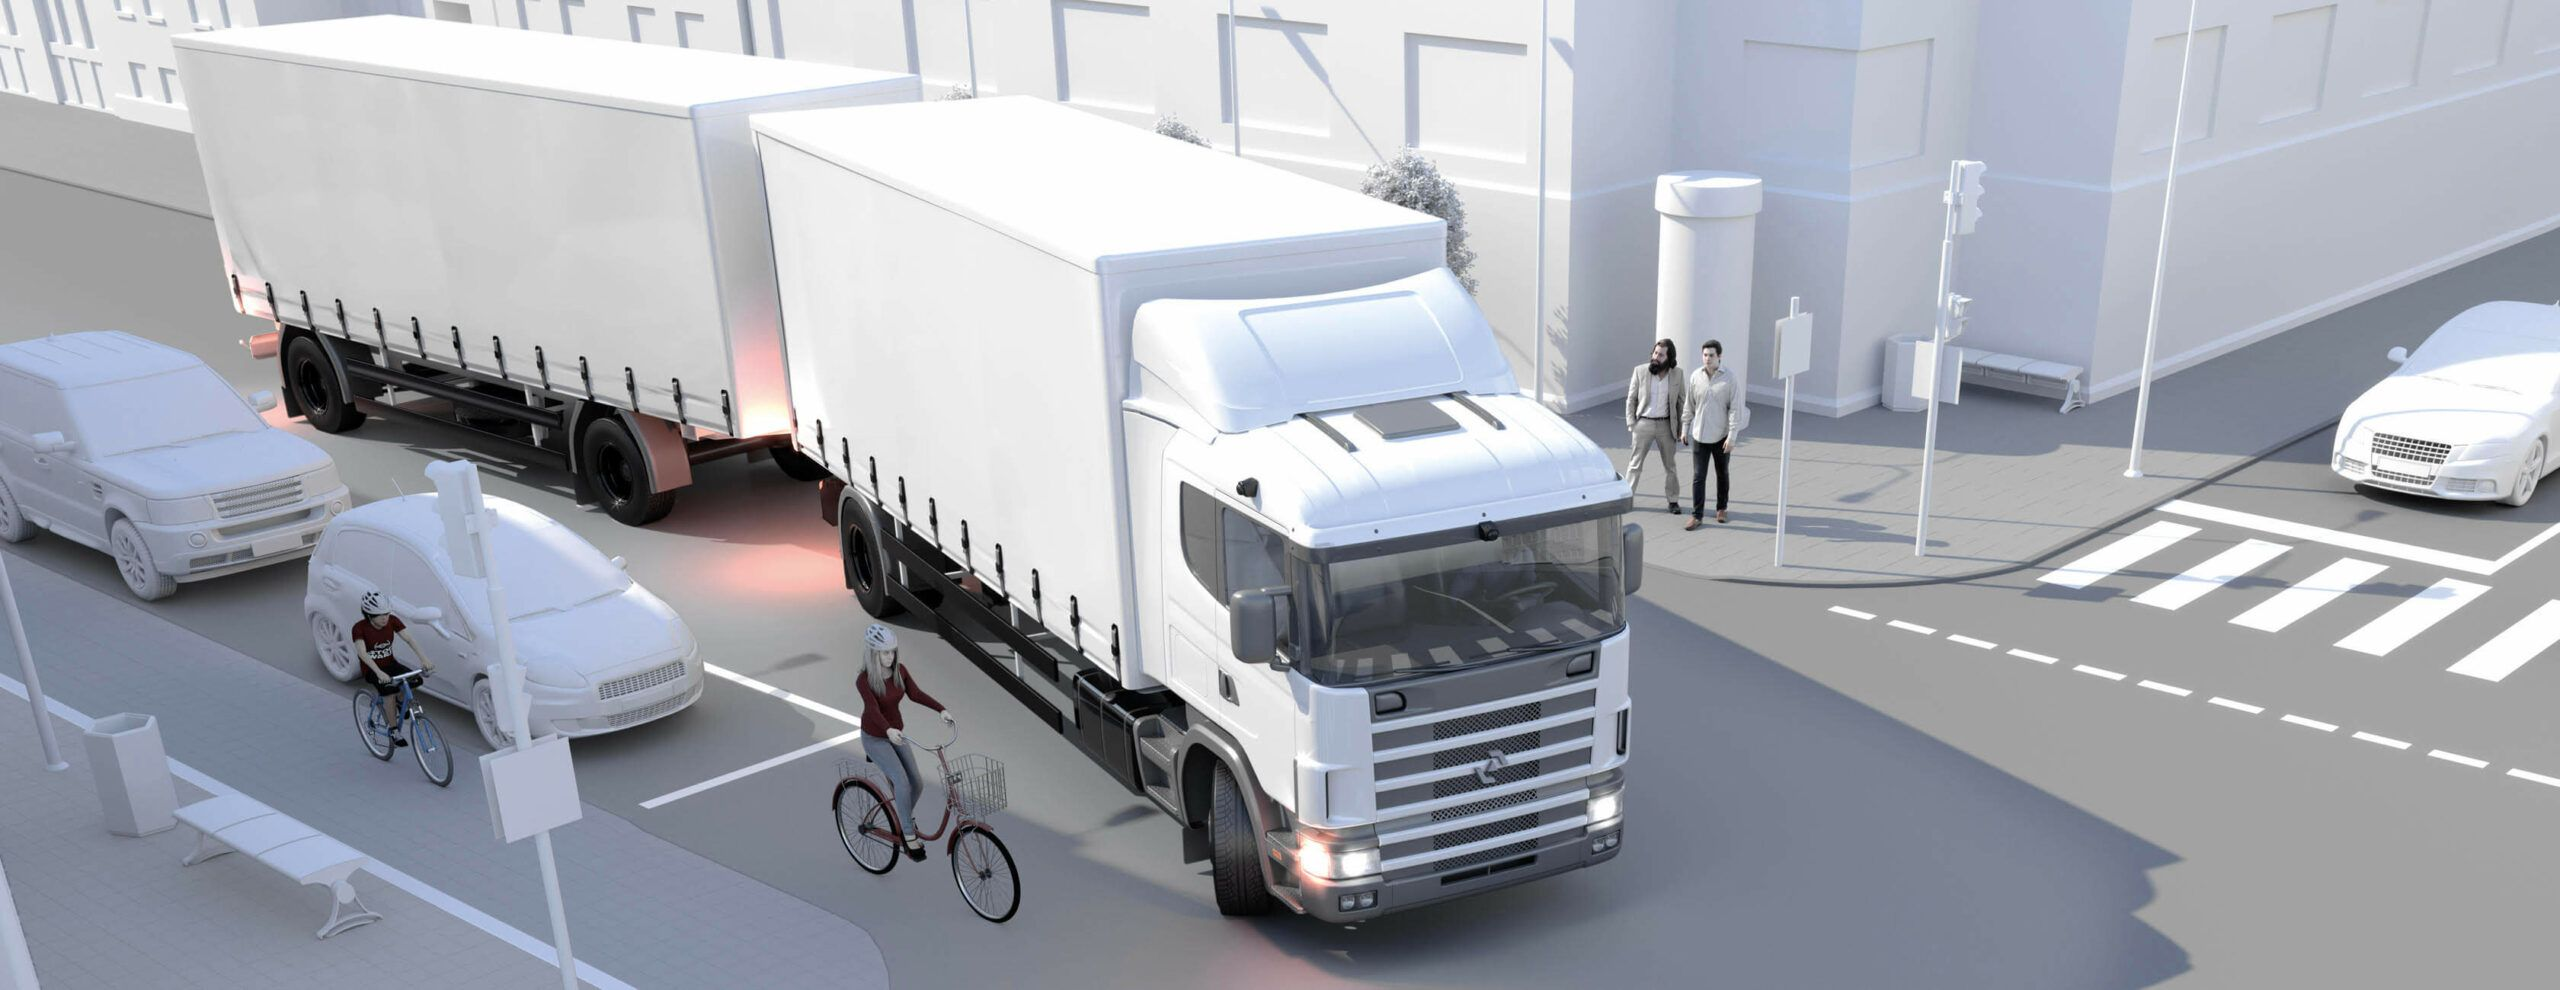
\includegraphics[width=1\linewidth]{images/abbiegeassistent-scaled-7b2478b8}\\[1ex]
    \centering
    \caption{Beispiel Rechtsabbiegen LKW}
    \label{ABBILDUNG}
\end{figure}


Eine besonders bedeutende Neuerung im Bereich der \acf{LKW}-Sicherheit stellen Abbiegeassistenten dar. 
Diese Systeme helfen, den toten Winkel zu reduzieren und somit Unfälle – insbesondere beim Rechtsabbiegen – zu vermeiden. 
Trotz dieser technischen Fortschritte besteht weiterhin Potenzial für weitere Verbesserungen. Eine umfassende Forschung und Entwicklung 
im Bereich von Fahrerassistenzsystemen könnte zukünftig dazu beitragen, das allgemeine Verkehrsrisiko weiter zu senken und die Verkehrssicherheit
signifikant zu erhöhen. \cite{SlightIncreaseNumber}

\clearpage

\subsection{Zielsetzung}
Zielsetzung dieser Studienarbeit ist es, einen 
leistungsfähigen Datenlogger zu entwickeln und die Visualisierung 
zu verbessern, um die Funktionalität des Fahrerassistenzsystems zu erhöhen 
und dadurch dessen Entwicklung zu erleichtern. Durch die Implementierung eines 
leistungsfähigen Datenloggers sollen Messwerte systematisch und zuverlässig 
erfasst werden können, was eine effektivere Zusammenarbeit im Entwicklungsteam 
ermöglicht und die Notwendigkeit einer dauerhaften Hardwareverbindung reduziert. Die Optimierung der Visualisierung 
dient dazu, Messergebnisse klarer und übersichtlicher darzustellen, um künftige Analysen und Tests zu vereinfachen und somit
 die Qualität und Genauigkeit der Positionsbestimmung zu erhöhen. Diese Verbesserungen sollen letztlich zu einer höheren Effizienz
  im Entwicklungsprozess führen und 
somit einen wesentlichen Beitrag zur Erhöhung der Verkehrssicherheit leisten.

\clearpage

\section{Rückblick auf das mobile Warnsystem}
\subsection{Konzept und Zielsetzung}
Die vorherige Studienarbeit verfolgte das Ziel, ein mobiles Warnsystem zur Minimierung von 
Abbiegeunfällen zwischen \ac{LKW} und ungeschützten Verkehrsteilnehmenden wie Fußgängerinnen und Radfahrerinnen zu entwickeln.
Zentrales Element dieses Systems war eine mobile Applikation, die als aktiver Bluetooth-Sender fungieren sollte. In Kombination 
mit einem am \ac{LKW} montierten Empfängerboard (basierend auf dem u-blox XPLR-AOA-1 Kit) sollte mithilfe der \acf{AoA}-Technologie 
die Position des Smartphones lokalisiert und bei drohender Gefahr eine Warnung ausgegeben werden. Das System versprach einen 
kostengünstigen und einfach zugänglichen Ansatz zur Verbesserung der Verkehrssicherheit im städtischen Raum.

\subsection{Bluetooth AoA und technische Grundlagen}
Die \acf{AoA}-Technologie ist Teil des Bluetooth 5.1-Standards und ermöglicht die Positionsbestimmung
eines Senders durch Messung des Einfallswinkels der Funksignale an mehreren Antennen eines Empfängers \cite{miller2021bluetooth,uBloxAoAWhitepaper}. 
Voraussetzung hierfür ist jedoch ein exakter Zugang zu den Bluetooth-Sendeparametern sowie eine Antennenkonfiguration 
mit bekannten geometrischen Abständen. Das u-blox XPLR-AOA-1 Explorer Kit stellt hierzu eine geeignete Hardwarelösung dar, 
da es mit einem \ac{AoA}-fähigen Empfängerboard und einem sogenannten Tag (Sender) ausgestattet ist. Ziel der Arbeit war es, das Smartphone 
funktional durch diesen Tag zu ersetzen.

\begin{figure}[H]
    \centering
    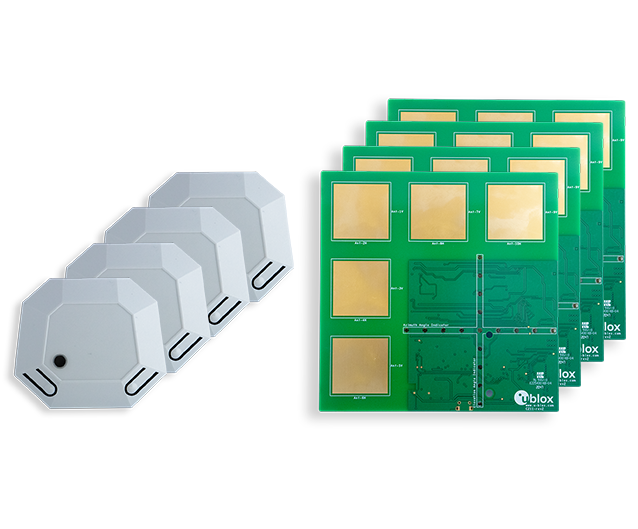
\includegraphics[width=1\linewidth]{images/XPLR-AOA-with-C209-and-C211-02_0}
    \caption{XPLR-AOA Explorer Kit}
    \label{ABBILDUNG}
\end{figure}

\subsection{Herausforderungen und Gründe für die Projektpause}
Im praktischen Verlauf der Umsetzung traten mehrere schwerwiegende technische Limitierungen auf, die die Fortführung des Projekts verhinderten:

\begin{itemize}
    \item Aktuelle Smartphone-Firmware (insbesondere auf Android-Basis) verhindert in der Regel den vollständigen Zugriff auf die Bluetooth-Sendeparameter. Ein gezieltes Emittieren von \acf{BLE}-Signalen, wie es zur \ac{AoA}-Ortung erforderlich ist, ist mit dem Standard-\acf{SDK} nicht möglich \cite{androidBLElimitation}.
    \item Nur wenige aktuelle Mobilgeräte unterstützen Bluetooth 5.1 vollständig, was die Reichweite und Genauigkeit der Ortung stark einschränkt \cite{ble51market2023}.
    \item Die Emulation des u-blox Tags durch das Smartphone scheiterte daher an mangelnden Systemrechten, fehlendem Low-Level-\acf{API}-Zugriff und nicht ausreichender Hardwareunterstützung.
\end{itemize}

Diese Faktoren führten dazu, dass das Projekt in der geplanten Form nicht abgeschlossen werden konnte. 
Die zugrundeliegende Idee bleibt jedoch vielversprechend und kann in Zukunft wieder aufgegriffen werden, sobald sich 
die technischen Rahmenbedingungen verbessert haben.

\clearpage

\section{Grundlagen Datenlogger}
\subsection{Zweck und Funktionalität eines Datenloggers}
Ein Datenlogger ist ein autonom arbeitendes Gerät oder Softwaremodul, das physikalische oder digitale Messwerte über einen definierten Zeitraum hinweg aufzeichnet. Ziel ist es, Veränderungen systematisch und zuverlässig zu erfassen, um sie später analysieren, auswerten oder dokumentieren zu können \cite{poole2020data, smith2018sensors}. Typische erfasste Daten umfassen beispielsweise Temperatur, Spannung, Zeitstempel, Lage- oder Positionsdaten.

\begin{figure}[H]
    \centering
    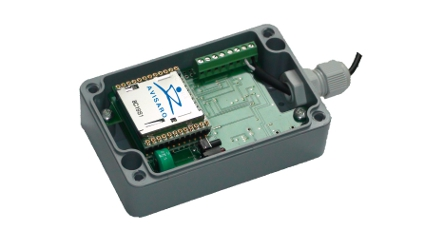
\includegraphics[width=1\linewidth]{images/Datalogger}
    \caption{Datenlogger Cube (Avisaro 2.0) zur Speicherung von Sensor- und Prozessdaten}
    \label{fig:datenlogger_cube}
\end{figure}

Im Gegensatz zu interaktiven Messsystemen arbeitet ein Datenlogger in der Regel unabhängig und ohne dauerhafte Verbindung zu einem Steuergerät. Dadurch eignet er sich besonders für mobile oder schwer zugängliche Anwendungen. Die kontinuierliche Aufzeichnung ermöglicht eine lückenlose Nachverfolgbarkeit, was insbesondere bei der Entwicklung, Fehlersuche und Validierung technischer Systeme von großer Bedeutung ist \cite{dewesoft2024guide}.

Wichtige Eigenschaften eines Datenloggers umfassen unter anderem eine ausreichende Speicherkapazität, eine hohe Energieeffizienz sowie die Kompatibilität zu standardisierten Datenformaten wie \ac{CSV} oder \ac{JSON}. Moderne Logger bieten darüber hinaus Schnittstellen für drahtlose Datenübertragung oder eine automatisierte Synchronisation mit Analysetools \cite{rs2022guide}.

\subsection{Anwendungsbereiche im Kontext der Studienarbeit}
Im Rahmen dieser Studienarbeit wird der Datenlogger gezielt eingesetzt, um die Entwicklungsarbeit am Bluetooth-\ac{AoA}-basierten Lokalisierungssystem effizienter und flexibler zu gestalten. Ziel ist es, die Abhängigkeit von einer aktiven Verbindung zur Hardware während der Test- und Anpassungsphasen zu minimieren \cite{poole2020data}. Personen, die an der Parametrierung oder Feinjustierung des Systems arbeiten, sollen in die Lage versetzt werden, auch ohne direkte Verbindung zur u-blox-Hardware auf reale Messdaten zuzugreifen.

Der Datenlogger dient dabei nicht nur der reinen Aufzeichnung, sondern ermöglicht die Speicherung von tatsächlich erfassten, originalgetreuen Messwerten. Diese Werte können anschließend in separate Programme oder Auswertungswerkzeuge importiert werden, um dort Berechnungen, Analysen und grafische Darstellungen durchzuführen. Änderungen an Parametern oder Auswertealgorithmen können somit auf Basis gespeicherter Daten vorgenommen und getestet werden, ohne dass dafür eine erneute Datenerfassung mit der realen Sensorik notwendig ist \cite{smith2018sensors}.

\begin{figure}[H]
    
\includegraphics[width=1\linewidth]{images/Flussdiagramm Datenlogger.png}\\[1ex]
    \centering
    \caption{Integration Datenlogger}
    \label{ABBILDUNG}
\end{figure}

Darüber hinaus erlaubt der Datenlogger eine „Offline-Simulation“ oder ein Daten-Replay mit echten Werten. Diese Vorgehensweise bietet den Vorteil, dass Optimierungen zunächst im Testsystem geprüft werden können. Erst wenn ein Ergebnis zufriedenstellend ist, wird es auf das reale System übertragen. Damit leistet der Datenlogger einen wesentlichen Beitrag zur Entkopplung von Entwicklung und Hardwareverfügbarkeit \cite{dwyer2015what}.

\subsection{Vorhandene Herausforderungen und Lösungsansätze}
Bei der Entwicklung eines zuverlässigen Datenloggers im Kontext des Bluetooth-\ac{AoA}-Systems treten verschiedene Herausforderungen auf. Eine der zentralen Schwierigkeiten liegt in der exakten zeitlichen Zuordnung der erfassten Daten. Für eine sinnvolle Auswertung müssen Zeitstempel, Empfangswinkel und weitere Messgrößen synchronisiert und konsistent gespeichert werden \cite{rs2022guide}.

Ein weiteres Problem stellt die effiziente und verlustfreie Speicherung großer Datenmengen dar. Hierbei müssen sowohl die Speicherkapazität als auch die Lesbarkeit und Weiterverwendbarkeit berücksichtigt werden. Gerade im Hinblick auf die spätere Analyse mit gängigen Tools wie Python oder MATLAB ist ein gut strukturiertes Datenformat – etwa \ac{CSV} oder \ac{JSON} – von hoher Bedeutung \cite{dewesoft2024guide}.

Auch die Integration in bestehende Entwicklungsprozesse erfordert eine durchdachte Schnittstellengestaltung. Der Datenlogger muss flexibel und modular aufgebaut sein, damit er problemlos in verschiedene Testumgebungen eingebunden werden kann. Gleichzeitig soll der Energieverbrauch möglichst gering gehalten werden, um auch den mobilen Einsatz über längere Zeiträume hinweg zu ermöglichen \cite{smith2018sensors}.

Lösungsansätze bestehen in der Verwendung eines einfachen, standardisierten Speicherformats, einem modularen Softwaredesign mit klar dokumentierten Schnittstellen sowie in der Implementierung grundlegender Fehlererkennungs- und Synchronisationsmechanismen. Diese Maßnahmen sollen sicherstellen, dass der Datenlogger zuverlässig, energieeffizient und nutzerfreundlich eingesetzt werden kann \cite{poole2020data}.

\clearpage

\section{Entwicklung des Datenloggers}
\subsection{Anforderungen an die Software}
Die zu entwickelnde Datenlogger-Software muss sich nahtlos in die bestehende Systemarchitektur integrieren lassen und gleichzeitig zentrale 
Anforderungen erfüllen: Dazu zählen eine robuste Speicherung relevanter Messdaten, flexible Möglichkeiten zur Wiederverwendung der Daten für 
Tests und Visualisierungen sowie eine einfache Wartbarkeit und Erweiterbarkeit des Codes.

Ein zentrales Ziel war die Entkopplung der Datenerfassung von der physischen Hardware. Durch die Offline-Nutzung gespeicherter Messdaten 
sollen Entwickler in die Lage versetzt werden, auch ohne Zugang zur u-blox-Hardware Analysen durchzuführen und Visualisierungen zu testen.

Darüber hinaus wurde eine klar strukturierte, leicht lesbare Datenhaltung gefordert, die eine spätere Auswertung und Visualisierung mit
gängigen Tools ermöglicht. Auch Mehrbenutzerfähigkeit und Plattformunabhängigkeit wurden als wünschenswerte Eigenschaften identifiziert.

\subsection{Auswahl geeigneter Technologien und Tools}
Die Softwarearchitektur wurde so gewählt, dass vorhandene Strukturen optimal weiterverwendet werden können. Die bestehende Kommunikation mit der 
u-blox-Hardware basiert auf einer performanten C++-Schicht, die beibehalten wurde. Neue Komponenten – insbesondere der Datenlogger und die Replay-Funktionalität – wurden hingegen in Python implementiert. Diese Kombination ermöglicht flexible Anpassungen bei geringem Änderungsaufwand, ohne die Stabilität des bestehenden Kerncodes in C++ zu beeinträchtigen. Diese Vorgehensweise bietet eine effiziente Balance zwischen Leistungsfähigkeit (via C++) und Entwicklungsproduktivität (via Python) \cite{cpp_python_integration}.

Zur Speicherung der Messdaten wurde das \ac{JSON}-Format ausgewählt. Dieses Format erlaubt eine strukturierte Ablage komplexer Datensätze, bestehend aus Zeitstempeln, \ac{AoA}-Winkeln, Signalstärken sowie weiteren Metadaten. Dies erlaubt eine maschinenlesbare und standardisierte Datenhaltung, die ideal für spätere Analysen geeignet ist \cite{json_logging_bestpractices}.

Durch diese Technologieentscheidung konnten die in Abschnitt 4.1 genannten Anforderungen erfüllt werden: Die Lösung ist plattformunabhängig,
 modular, nachvollziehbar und unterstützt eine effiziente Weiterentwicklung sowie Zusammenarbeit im Team.

\subsection{Implementierung und Integration in bestehende Systeme}

Die Implementierung des Datenloggers erfolgte im Rahmen eines bestehenden Lokalisierungssystems, das auf der Bluetooth-\ac{AoA}-Technologie 
basiert. Ziel war es, die Erfassung, Speicherung und spätere Analyse von Messwerten so zu gestalten, dass diese unabhängig
von einer Live-Hardwareverbindung möglich ist und flexibel in den Entwicklungsprozess integriert werden kann.

\paragraph{Messung – Entstehung der Rohdaten}

Im Zentrum der Messung stehen zwei Hauptkomponenten: das sogenannte Tag, das als zu verfolgendes Objekt fungiert 
und kontinuierlich Signale sendet, sowie mindestens zwei Anker (Anchors), die als fest installierte Empfangseinheiten dienen. 
Die Anker, ausgestattet mit mehreren Antennen, empfangen das Signal des Tags und bestimmen den Einfallswinkel (\ac{AoA}), unter dem 
das Signal ankommt. 

\paragraph{Datenerfassung und -aufbereitung}

Die Kommunikation zwischen Ankern und Rechner erfolgt typischerweise über eine serielle Schnittstelle oder \ac{BLE}. 
Ein Python-Skript (z.\,B. \texttt{getAnchorData.py}) liest die Rohdaten kontinuierlich aus. Für jede einzelne Messung werden strukturierte Informationen
erfasst, darunter:

\begin{itemize}
    \item \texttt{anchors}: Positionen der Anker, z.\,B. \texttt{[[3, 0], [0, 0]]}
    \item \texttt{angles}: Die gemessenen Winkel, z.\,B. \texttt{[-31, 24]}
    \item \texttt{sensor\_values}: Eine Liste weiterer Sensordaten:
\begin{lstlisting}[language=]
[
  {"theta": 90, "val": -31, "pos": [3, 0], "speed_along_line": 0, "risk_level": 1},
  {"theta": 90, "val": 24, "pos": [0, 0], "speed_along_line": 0, "risk_level": 1}
]
\end{lstlisting}
\end{itemize}

Die Daten werden zeilenweise im \ac{JSON} Lines-Format (\texttt{.jsonl}) gespeichert. Jede Zeile enthält einen Zeitstempel und die zugehörigen Sensordaten. 
Ein Beispiel für eine gespeicherte Messung ist:

\begin{verbatim}
{"timestamp": "2025-06-03T06:32:50.140342", 
 "raw_sensor_data": {
   "anchors": [[3, 0], [0, 0]], 
   "angles": [-31, 24], 
   "sensor_values": [...]
 }}
\end{verbatim}

\paragraph{Berechnung der Tag-Position – Triangulation}

Aus den gemessenen Winkeln und bekannten Positionen der Anker wird die Position des Tags durch Triangulation berechnet. Jeder Anker 
definiert eine Gerade, auf der sich der Tag befinden könnte. Die Schnittpunktberechnung dieser Geraden liefert eine Positionsschätzung. Die Richtung 
jeder Linie ergibt sich aus dem gemessenen Winkel mittels:

\[
dx = \sin(\theta), \quad dy = \cos(\theta)
\]

Der Schnittpunkt wird mithilfe der folgenden Gleichung bestimmt:

\[
t_1 = \frac{(x_2 - x_1) \cdot dy_2 - (y_2 - y_1) \cdot dx_2}{dx_1 \cdot dy_2 - dy_1 \cdot dx_2}
\]

und

\[
x = x_1 + t_1 \cdot dx_1, \quad y = y_1 + t_1 \cdot dy_1
\]

Diese Berechnung kann sowohl live während der Datenerfassung als auch im Nachgang im sogenannten Replay-Modus erfolgen.

\vspace{1em}
\textbf{Legende zur Formel:}
\begin{itemize}
    \item $x_1, y_1$: Koordinaten des ersten Ankers
    \item $x_2, y_2$: Koordinaten des zweiten Ankers
    \item $\theta_1, \theta_2$: Empfangene Winkelinformationen (\ac{AoA}) an Anker 1 bzw. Anker 2
    \item $dx_1, dy_1$: Richtungsvektor vom ersten Anker, berechnet mit $\sin(\theta_1), \cos(\theta_1)$
    \item $dx_2, dy_2$: Richtungsvektor vom zweiten Anker analog dazu
    \item $t_1$: Skalierungsfaktor entlang der Linie des ersten Ankers zur Schnittpunktberechnung
    \item $x, y$: Berechnete Position des Tags im zweidimensionalen Raum
\end{itemize}

\begin{figure}[H]
    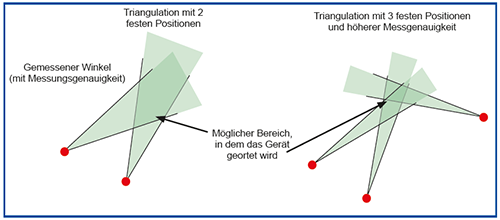
\includegraphics[width=1\linewidth]{images/1906_abbildung1 (1)}\\[1ex]
    \centering
    \caption{Beispiel Triangulation}
    \label{ABBILDUNG}
\end{figure}

\paragraph{Speicherung und Weiterverarbeitung}

Sämtliche berechneten Werte – Winkel, Position, Sensordaten – werden chronologisch gespeichert. Das Python-Skript \texttt{replayLogger.py} 
ermöglicht das Einlesen dieser Datei und berechnet bei Bedarf die Position erneut. Dies erlaubt eine erneute Analyse oder die Anwendung überarbeiteter 
Algorithmen.

\paragraph{Nachträgliche Optimierung der Rechenlogik}

Während der frühen Entwicklungsphase bestand ein grundlegendes Problem darin, dass beim Replay die gespeicherten Daten lediglich wiedergegeben wurden, wie sie während der ursprünglichen Messung aufgezeichnet worden waren. Das bedeutete, dass keine Neuberechnung der Tag-Position erfolgte – Anpassungen an Parametern oder Algorithmen blieben somit wirkungslos. 

Im weiteren Verlauf wurde dieser Fehler behoben. Das Replay-Modul (\texttt{replayLogger.py}) wurde so erweitert, dass beim Einlesen der Logdaten die gespeicherten Rohwerte wie Winkel und Ankerpositionen erneut verarbeitet werden. Auf diese Weise erfolgt bei jedem Replay eine aktuelle Berechnung der Position mittels Triangulation. Dadurch können Änderungen in der Positionsberechnung zunächst rein softwareseitig überprüft und validiert werden – ganz ohne Hardwareeinsatz. Nach erfolgreicher Evaluierung lassen sich die neuen Parameter und Berechnungsverfahren schließlich in das Echtzeit-Tracking-System übernehmen.

\paragraph{Visualisierung der Messdaten}

Der Datenlogger stellt über eine \acf{TCP}-Verbindung eine Schnittstelle zur grafischen Visualisierung her (durch das Skript \texttt{ui.py}). 
Jede Messung wird als \ac{JSON}-Objekt an die Benutzeroberfläche übertragen und enthält neben der berechneten Position auch zugehörige Sensordaten. 
Die Benutzeroberfläche stellt folgende Informationen dar:

\begin{itemize}
    \item Die aktuelle Position des Tags
    \item Visualisierte Anker (Empfängerboards) 
    \item Zusatzinformationen wie Bewegung oder Risikobewertung
\end{itemize}

\paragraph{Zusammenfassung des Datenflusses}

Der vollständige Ablauf lässt sich wie folgt beschreiben:

\begin{enumerate}
    \item \textbf{Messung:} Anker empfangen Signale und bestimmen Winkel sowie Sensordaten.
    \item \textbf{Datenerfassung:} Python-Skripte lesen die Daten aus und speichern sie als \ac{JSONL}.
    \item \textbf{Speicherung:} Die Daten werden zeilenweise mit Zeitstempel archiviert.
    \item \textbf{Replay:} Ein weiteres Skript liest die Daten, berechnet ggf. die Position und sendet sie weiter.
    \item \textbf{Visualisierung:} Eine Benutzeroberfläche stellt Position und Sensordaten visuell dar.
\end{enumerate}

\begin{figure}[H]
    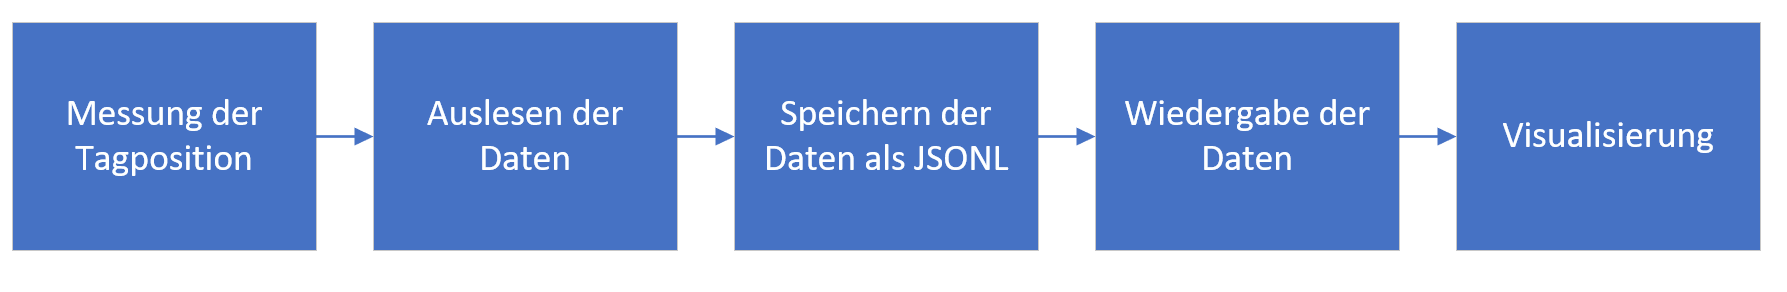
\includegraphics[width=1\linewidth]{images/Ablauf Funktion Datenlogger.png}\\[1ex]
    \centering
    \caption{Ablauf Funktion Datenlogger}
    \label{ABBILDUNG}
\end{figure}

\paragraph{Beispiel einer vollständigen Messung}

\begin{itemize}
    \item Anker 1: Winkel = \(-31^\circ\), Position = [3, 0]
    \item Anker 2: Winkel = \(24^\circ\), Position = [0, 0]
\end{itemize}

\textbf{Speicherung:}
\begin{verbatim}
{"timestamp": "...", 
 "raw_sensor_data": {
   "anchors": [[3, 0], [0, 0]], 
   "angles": [-31, 24], 
   "sensor_values": [...]
 }}
\end{verbatim}

\textbf{Replay:}  
Der Datenlogger berechnet erneut die Position und sendet z.\,B.:

\begin{verbatim}
{"point": {"position": [x, y], "Uncertainty": 0}, 
 "sensor_values": [...]}
\end{verbatim}

\textbf{Visualisierung:}  
Die Benutzeroberfläche zeigt Position, Bewegung und Risikobewertung an.

\paragraph{Fazit}

Durch die Trennung von Messung, Speicherung, Wiederverwendung und Visualisierung wurde ein System geschaffen, 
das sowohl im Live-Betrieb als auch für Offline-Analysen geeignet ist. Die Nutzung des \ac{JSONL}-Formats gewährleistet einfache 
Nachverarbeitung und hohe Transparenz im Entwicklungsprozess.

\subsection{Ergebnisse und Evaluation}

Die Implementierung des Datenloggers konnte erfolgreich in die bestehende Systemumgebung integriert werden. Die Erweiterung 
erfolgte durch ein einzelnes, in Python geschriebenes Modul, das mit nur wenigen Anpassungen in den vorhandenen Code eingebunden wurde. 
Diese modulare Herangehensweise ermöglichte eine einfache Integration, ohne die Stabilität der bestehenden C++- und Python-Strukturen zu beeinträchtigen.

Der Datenlogger ist in der Lage, strukturierte Messdaten zuverlässig zu erfassen, im \ac{JSONL}-Format zu speichern und diese in der 
\texttt{replayLogger.py} zur erneuten Verarbeitung und Visualisierung bereitzustellen. Durch die gezielte Nachberechnung der gespeicherten 
Parameter kann die Parametrisierung und Optimierung der Tag-Ortung nun auch ohne aktiven Hardwarezugang erfolgen. Dies stellt einen wesentlichen
 Fortschritt gegenüber früheren Ansätzen dar, bei denen für jede Änderung eine Live-Verbindung zur u-blox-Hardware erforderlich war.

Zur weiteren Erleichterung der Nutzung wurde eine \acf{BAT}-Datei erstellt, die den Datenlogger automatisch 
startet und eine benutzerfreundliche Auswahl der abzuspielenden Daten ermöglicht. Dadurch können mehrere aufgezeichnete Datensätze
 parallel gespeichert, umbenannt und bei Bedarf erneut abgespielt werden. Dies erleichtert sowohl die Organisation als auch die Wiederverwendbarkeit
  der Messdaten erheblich.

Die Kommunikation zwischen Logger und Visualisierung über \ac{TCP} funktioniert stabil, sodass eine Echtzeit- oder zeitnahe Darstellung 
der Messdaten in der grafischen Oberfläche möglich ist. Die Darstellung der Ergebnisse im \acf{UI} (Visualisierung) ist erfolgreich umgesetzt worden; die gespeicherten
 Positions- und Sensordaten lassen sich korrekt laden und werden visuell ansprechend aufbereitet.

\begin{figure}[H]
    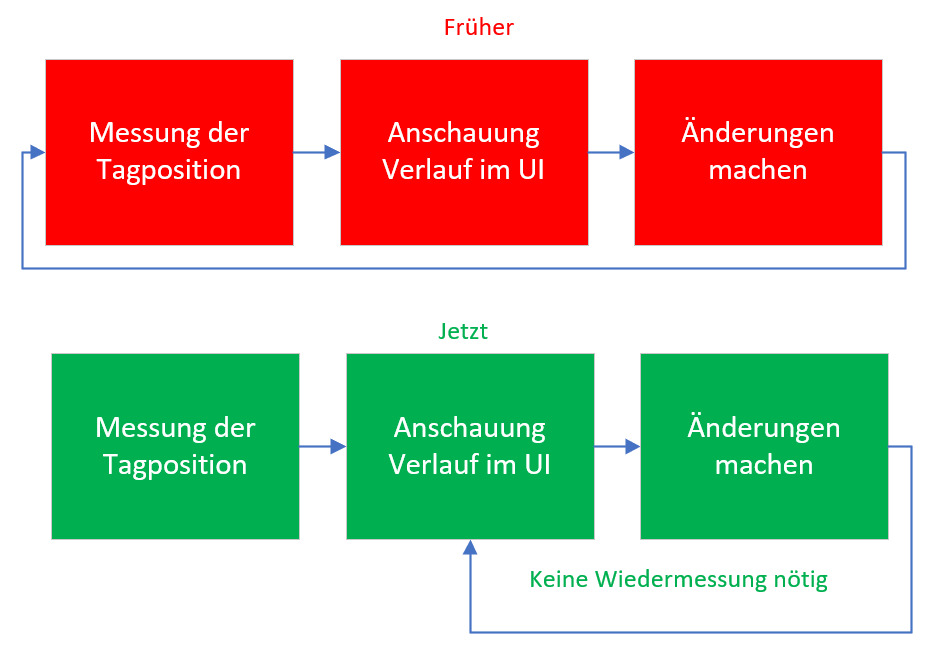
\includegraphics[width=1\linewidth]{images/Vergleich Parametrisierung.png}\\[1ex]
    \centering
    \caption{Vergleich Parametrisierung früher und heute}
    \label{ABBILDUNG}
\end{figure}

Ein weiterer Vorteil liegt in der verbesserten Teamfähigkeit des Systems. Da echte Messwerte gespeichert und wiederverwendet werden können, 
ist eine parallele Bearbeitung durch mehrere Teammitglieder möglich – unabhängig von der Verfügbarkeit der physischen Hardware.

Aktuell wurden nur kurze bis mittellange Messreihen (mehrere Minuten) getestet, die zuverlässig aufgezeichnet und verarbeitet werden konnten. 
Für den produktiven Einsatz müssen jedoch noch weiterführende Tests mit längeren Aufzeichnungen durchgeführt werden, um Speicherstabilität und 
Verarbeitungsgeschwindigkeit auch bei größeren Datenmengen zu validieren.

Insgesamt bildet der Datenlogger eine stabile Grundlage für künftige Entwicklungs- und Testarbeiten und ermöglicht sowohl effizientere als auch 
hardwareunabhängige Validierungsprozesse.

\section{Grundlagen der Visualisierung}
\subsection{Anforderungen an eine effektive Visualisierung}

Die visuelle Darstellung von Mess- und Sensordaten spielt eine zentrale Rolle bei der Entwicklung technischer Systeme. 
Im Kontext dieser Studienarbeit soll die Visualisierung nicht nur als Ausgabeinstrument dienen, sondern als aktives Analysewerkzeug die 
Entwicklung des Fahrerassistenzsystems unterstützen. Daraus ergeben sich spezifische Anforderungen an Struktur, Funktionalität und Performance der 
Visualisierung.

Ein wesentliches Kriterium ist die \textbf{Klarheit und Verständlichkeit} der Darstellung. Die Position des zu 
verfolgenden Objekts (Tag), die Winkelmessungen sowie weitere Sensordaten wie Geschwindigkeit oder Risikoindikatoren müssen 
für die Benutzer klar erkennbar und intuitiv interpretierbar sein. Die gewählte Darstellungsform darf keine zusätzliche Komplexität 
einführen, sondern soll das Verständnis der Systemdynamik fördern \cite{tkinter_guidelines}.

Zudem ist \textbf{Reaktionsfähigkeit} von hoher Bedeutung. Insbesondere bei der Wiedergabe von Logdaten im Replay-Modus ist sicherzustellen, 
dass Positionsdaten und Zustandsänderungen nahezu in Echtzeit visualisiert werden, ohne spürbare Verzögerung oder Datenverluste. Dies ist entscheidend
für die genaue Nachverfolgung zeitkritischer Situationen und zur Validierung der Algorithmen \cite{realtime_visualization}.

Eine \textbf{strukturierte und modulare Darstellung} ermöglicht es, verschiedene Datenebenen simultan darzustellen. 
Dazu gehören beispielsweise die grafische Repräsentation von Ankerpositionen, Trajektorien, Messwinkeln sowie Risikoabschätzungen in Form von 
Farbcodierungen, Symbolen oder Vektorpfeilen. Die visuelle Trennung dieser Elemente soll die Lesbarkeit erhöhen und gleichzeitig Korrelationen zwischen 
den Daten sichtbar machen.

Weiterhin ist \textbf{Flexibilität} in der Konfiguration erforderlich. Die Visualisierung soll es ermöglichen, verschiedene Parameter 
anzupassen oder unterschiedliche Datensätze zu vergleichen. Auf diese Weise können gezielte Analysen durchgeführt und das Verhalten 
des Systems unter unterschiedlichen Bedingungen besser nachvollzogen werden.

Die Software muss zudem eine \textbf{hohe Stabilität und Performance} aufweisen. Auch bei großen Datenmengen oder längeren Wiedergaben dürfen keine 
Speicherprobleme oder Verzögerungen auftreten. Gleichzeitig soll der Ressourcenverbrauch moderat bleiben, um eine Nutzung auf Standardhardware zu 
gewährleisten.

Darüber hinaus ist die \textbf{Schnittstellenkompatibilität} entscheidend. Die Visualisierung kommuniziert über eine \ac{TCP}-Verbindung mit dem Datenlogger 
und verarbeitet strukturierte \ac{JSON}-Daten. Sie muss in der Lage sein, kontinuierlich neue Informationen entgegenzunehmen, korrekt zu interpretieren und 
grafisch darzustellen \cite{tcp_json_integration}.

Schließlich sollte die Visualisierung eine \textbf{benutzerfreundliche Interaktion} bieten. Die Bedienoberfläche muss auch für neue Projektmitglieder 
oder externe Tester leicht verständlich sein. Eine klare Struktur und einfache Bedienlogik erhöhen die Zugänglichkeit und 
erleichtern die Nutzung im Entwicklungsteam.

\subsection{Darstellungsmöglichkeiten und -technologien}

Die grafische Darstellung von Messergebnissen ist ein zentrales Element zur Analyse, Entwicklung und Validierung des Fahrerassistenzsystems.
Ziel der Visualisierung ist es, komplexe Daten wie Winkelmessungen, berechnete Positionen und Sensordaten so aufzubereiten, dass sie schnell
erfasst und zielgerichtet interpretiert werden können.

\paragraph{Darstellungsformen}

Für die Anforderungen dieses Projekts wurde eine zweidimensionale Darstellung gewählt. In einem kartesischen Koordinatensystem werden sowohl 
die festen Positionen der Anker als auch die berechnete Position des Tags eingezeichnet. Zur Darstellung zusätzlicher Informationen, 
wie beispielsweise der Risikobewertung, kommt eine Farbcodierung zum Einsatz: Grün signalisiert eine sichere Entfernung, Gelb eine 
Warnsituation und Rot eine mögliche Kollisionsgefahr.

Auch die Darstellung der Sensordaten erfolgt visuell, etwa durch Richtungslinien oder Symbole, die Informationen wie potenzielle 
Gefahrenzonen oder die Antennenausrichtung übermitteln.

Zur besseren Nachvollziehbarkeit der Messabläufe wurden Replays implementiert, mit denen frühere Positionen nacheinander dargestellt 
werden können. Diese Funktion unterstützt nicht nur die Analyse von Bewegungsmustern, sondern ermöglicht auch eine gezielte Anpassung 
der Systemparameter sowie eine anschauliche Präsentation auf Messen oder in Testumgebungen.

\paragraph{Technologische Umsetzung}

Für die technische Realisierung wurde Python als Basissprache verwendet, da es bereits im bestehenden Projektumfeld (z.\,B. Datenlogger, \ac{TCP}-Client)
genutzt wird und eine einfache Integration von Visualisierungs- und Netzwerkmodulen ermöglicht. Die grafische Benutzeroberfläche basiert auf \texttt{Tkinter}
und nutzt ein Zeichenfenster (\texttt{Canvas}), das dynamisch aktualisiert wird, um Positionen, Sensorrichtungen und Kontextinformationen darzustellen \cite{tkinter_book}.

Zur Anzeige der Daten kommen vor allem folgende Technologien zum Einsatz:

\begin{itemize}
    \item \textbf{Tkinter:} Zur Umsetzung der grafischen Oberfläche, inklusive dynamischer Zeichnung von Positionen, Sensoren und Symbolen \cite{tkinter_book}.
    \item \textbf{TCP-Kommunikation:} Die Visualisierung empfängt die Daten über eine \ac{TCP}-Verbindung, die vom Datenlogger bereitgestellt wird (Skript \texttt{ui.py}) \cite{tcp_json_integration}.
    \item \textbf{JSON-Verarbeitung:} Die Logdateien und Echtzeitdaten liegen im \ac{JSON}-Format vor und werden zur Laufzeit dekodiert \cite{json_processing_books}.
\end{itemize}

Der Aufbau der Visualisierung ist modular gehalten, sodass zukünftige Änderungen – etwa am Format der Sensordaten oder an der
Positionsberechnung – ohne tiefgreifende Eingriffe umgesetzt werden können.

\paragraph{Schnittstellen und Erweiterbarkeit}

Die Benutzeroberfläche ist so gestaltet, dass verschiedene Datenquellen unterstützt werden: Neben Live-Daten aus dem Logger ist auch ein 
Replay-Modus möglich, in dem ältere Messungen abgespielt werden. Dies wird durch einen einfachen Startbefehl (über eine Batch-Datei oder
Kommandozeilenparameter) gesteuert.

Die Datenstruktur aus der \ac{JSONL}-Datei ermöglicht eine verlustfreie Weiterverarbeitung der gespeicherten Informationen. Durch die Trennung von 
Backend (Logger/Replay) und Frontend (Visualisierung) ist das System erweiterbar. Eine spätere Portierung auf fortgeschrittenere GUI-Frameworks 
(z.\,B. \texttt{PyQt} oder webbasierte Tools wie \texttt{Plotly Dash}) ist ebenso denkbar wie eine Erweiterung auf 3D-Darstellungen 
mithilfe von OpenGL oder Unity.

\paragraph{Optionale Abbildungsempfehlung}

Eine illustrative Abbildung könnte den schematischen Ablauf der Datenvisualisierung zeigen – von der Messung über die Speicherung bis zur Anzeige. 
Beispielhaft könnte sie folgende Elemente enthalten:

\begin{itemize}
    \item Position der Anker (als fixe Punkte)
    \item Messwinkel (als Linien vom Anker ausgehend)
    \item Position des Tags (als Punkt mit Zeitstempel)
    \item Risikobewertung als Farbring oder Symbol
    \item Spurverlauf der Tag-Position (z.\,B. gestrichelte Linie)
\end{itemize}

Eine solche schematische Darstellung erleichtert das Verständnis des Visualisierungskonzepts auch für fachfremde Leserinnen und Leser.

\paragraph{Fazit}

Die gewählten Technologien und Darstellungsformen ermöglichen eine performante, verständliche und flexible Visualisierung der Messergebnisse. Sie 
bilden damit eine wichtige Grundlage für die weiterführende Analyse, Parametrisierung und Validierung des Fahrerassistenzsystems.

\section{Entwicklung der neuen Visualisierung}
\subsection{Analyse der bestehenden Visualisierung}

Die bisherige grafische Benutzeroberfläche (\ac{UI}) wurde in Python entwickelt und diente der Echtzeitdarstellung der aus dem Bluetooth-\ac{AoA}-System ermittelten
Tag-Position. Als zentrales Element wurde ein zweidimensionales kartesisches Koordinatensystem verwendet, innerhalb dessen ein einzelner Punkt die 
Bewegung des Tags repräsentierte. Die Position dieses Punktes wurde entweder durch eine direkte Live-Messung mit der Hardware oder durch eine 
vereinfachte Simulation erzeugt – eine Möglichkeit zur Wiederverwendung gespeicherter Daten durch einen Datenlogger war zu diesem Zeitpunkt noch nicht
implementiert \cite{tkinter_book}.

\begin{figure}[H]
    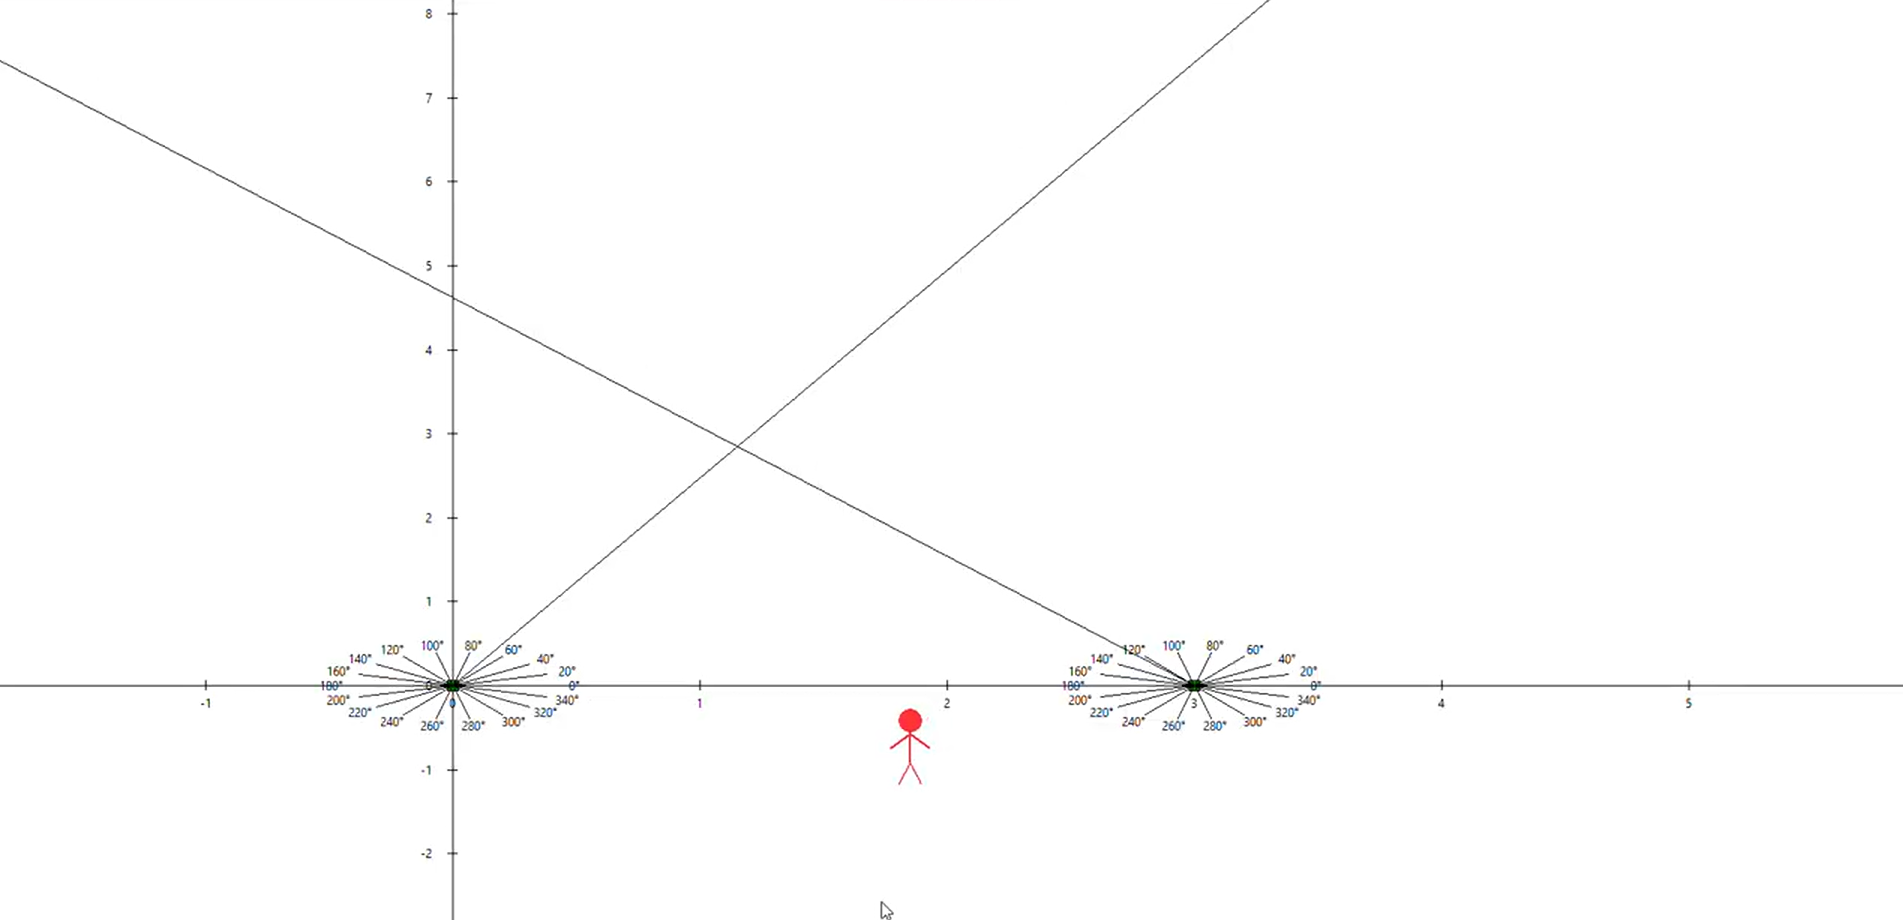
\includegraphics[width=1\linewidth]{images/Alte Visualisierung.png}\\[1ex]
    \centering
    \caption{Alte Visualisierung}
    \label{ABBILDUNG}
\end{figure}

Zur besseren Nachvollziehbarkeit der geometrischen Zusammenhänge wurden auch die fest installierten Empfangseinheiten (Anker) im Koordinatensystem 
visualisiert. Von deren Positionen ausgehend wurden Linien gezeichnet, welche die gemessenen Einfallswinkel (\ac{AoA}) darstellten. Die 
Idee dahinter war, die Triangulation – also die Schnittpunktberechnung zweier Richtungslinien – visuell darzustellen und die damit berechnete Tag-Position
zu validieren.

Allerdings wies diese Darstellung mehrere funktionale und darstellerische Einschränkungen auf. Eine grundlegende Schwäche bestand darin, dass der 
dargestellte Schnittpunkt der Winkel-Linien oft nicht exakt mit dem angezeigten Punkt des Tags übereinstimmte. Dies führte zu Inkonsistenzen, die 
insbesondere bei der Bewertung der Lokalisierungsgenauigkeit zu Verwirrung führen konnten.

Darüber hinaus fehlten wichtige Interaktionsmöglichkeiten und Darstellungsmodi: Sensorwerte oder Risikobewertungen konnten 
nicht separat angezeigt oder analysiert werden. Eine Zeitschrittsteuerung oder ein Replay-Modus waren nicht vorhanden. Da der 
Datenlogger zum damaligen Zeitpunkt noch nicht existierte, beschränkte sich die Funktionalität der Oberfläche auf Live-Datenströme oder manuell 
eingespeiste Simulationsdaten.

Zusammenfassend war die ursprüngliche Visualisierung funktional auf das Wesentliche reduziert, ermöglichte aber weder eine tiefere Analyse noch eine 
Nachbearbeitung historischer Messdaten. Die Einführung des Datenloggers \cite{json_processing_books} und eine verbesserte Visualisierung sollen diese Defizite beheben und eine 
fundierte, nachvollziehbare sowie interaktive Darstellung aller relevanten Systemparameter ermöglichen.

\subsection{Konzept einer verbesserten Visualisierung}

Basierend auf der Analyse der bisherigen Darstellung ergeben sich mehrere Ansatzpunkte für eine funktional und ästhetisch verbesserte Visualisierung
der Tag-Ortung. Ziel ist es, die Ausgabe so zu gestalten, dass auch technisch weniger versierte Personen – beispielsweise Besucher auf Messen oder 
Mitglieder in interdisziplinären Projektteams – intuitiv die Funktionsweise und Aussagekraft des Fahrerassistenzsystems nachvollziehen können \cite{human_factors_vis}.

Ein zentrales Element der neuen Visualisierung ist die verbesserte Darstellung des Tags. Bisher wurde dieser lediglich als bewegender Punkt im 
Koordinatensystem dargestellt, was der realen Anwendung – z.\,B. einem Fußgänger oder Fahrradfahrer im Straßenverkehr – kaum gerecht wurde. Zukünftig 
soll der Tag durch ein erkennbares Modell wie etwa eine stilisierte menschliche Figur (z.\,B. ein Stickman) ersetzt werden. Zusätzlich ist vorgesehen,
visuelle Elemente wie ein \ac{LKW}-Modell in die Darstellung zu integrieren, um die reale Gefahrenlage bei Abbiegesituationen plausibler zu simulieren.

Zur Verbesserung der Verständlichkeit soll die Bewegung des Tags flüssiger und zeitlich realistischer erfolgen. In der bisherigen Version war die 
Bewegung teils sprunghaft oder verzögert, was eine genaue Nachverfolgung erschwerte. Durch optimierte Synchronisation mit 
den übermittelten Messwerten soll die visuelle Bewegung stärker der tatsächlichen Bewegung des realen Objekts entsprechen.

Darüber hinaus ist geplant, ein interaktives Interface mit zusätzlichen Informationen bereitzustellen. So sollen Parameter wie Winkel, 
Positionskoordinaten oder Risikoindikatoren dynamisch eingeblendet und aktualisiert werden können – ein wesentliches Werkzeug für Entwickler bei der Fehleranalyse und Parametrierung \cite{usercentered_visualization}.

Ein weiterer Aspekt der verbesserten Darstellung betrifft das bisher fest eingeblendete Koordinatensystem. Dieses war zwar funktional nützlich,
beeinträchtigte jedoch stellenweise die Lesbarkeit und ästhetische Wirkung der grafischen Oberfläche – insbesondere bei öffentlichkeitswirksamen 
Präsentationen oder auf begrenzten Anzeigeflächen. Künftig soll daher eine Option implementiert werden, das Koordinatensystem bei Bedarf auszublenden 
oder gezielt ein- und auszublenden (Toggle-Funktion). Dies erlaubt eine flexiblere Darstellung und steigert die Übersichtlichkeit – insbesondere wenn 
die rein visuelle Wahrnehmung im Vordergrund stehen soll.

Insgesamt verfolgt das neue Visualisierungskonzept das Ziel, eine Brücke zwischen technischer Präzision und intuitiver Darstellbarkeit zu schlagen \cite{usercentered_visualization}. 
Es soll nicht nur die Qualität der Entwicklung verbessern, sondern auch die Kommunikation der Systemfunktionalität nach außen erleichtern – etwa in 
Präsentationen, bei Tests oder in zukünftigen Anwenderstudien.

\subsection{Implementierung der verbesserten Visualisierung}

Zur besseren Nachvollziehbarkeit der gemessenen Bewegungsdaten und zur verständlichen Darstellung des Systems für technische wie nicht-technische 
Betrachter wurde die Benutzeroberfläche (\ac{UI}) umfassend überarbeitet. Die Implementierung erfolgte in Python unter Verwendung des 
\texttt{tkinter}-Frameworks, wodurch eine flexible und plattformunabhängige grafische Visualisierung ermöglicht wurde \cite{tkinter_book}.

\paragraph{Grundstruktur und Aufbau}

Die Benutzeroberfläche besteht aus einem zentralen Zeichenbereich (Canvas), auf dem die Bewegung des zu lokalisierenden Objekts (Tag) visualisiert wird. 
Ergänzt wird dieser durch eine Steuerleiste am unteren Rand zur Interaktion (z.\,B. Start/Stop der Visualisierung oder Ein-/Ausblenden von Antennendaten) 
sowie einer Informationsleiste zur Anzeige der aktuellen Position und Zusatzdaten.

Die Visualisierung ist in mehreren Schichten aufgebaut:
\begin{itemize}
    \item Darstellung des Tags als dynamisch skalierbare Figur (z.\,B. Stickman oder Fahrzeugabbildung)
    \item Hintergrundkoordinatensystem mit optional einblendbaren Achsen und Skalen
    \item Einblendung der Position und Orientierung der Antennenarrays sowie der zugehörigen Messrichtungen (\ac{AoA}-Linien)
\end{itemize}

\paragraph{Verarbeitung eingehender Daten}

Die Visualisierung kommuniziert über eine \ac{TCP}-Verbindung mit dem Datenlogger, der kontinuierlich strukturierte \ac{JSON}-Datenpakete sendet. Diese enthalten 
Informationen zur geschätzten Position des Tags, Sensordaten sowie Metainformationen. Eine dedizierte Serverkomponente in der \ac{UI} nimmt die Daten entgegen,
extrahiert relevante Parameter und aktualisiert die grafische Darstellung entsprechend.

Zur Verbesserung der Darstellung wurde ein Glättungsverfahren mit exponentiellem Filter implementiert, um Positionssprünge durch Rauschen oder Ausreißer 
zu reduzieren \cite{signal_filtering}. Gleichzeitig werden unrealistische Sprünge oder abrupte Änderungen durch Grenzwerte abgefangen.

\paragraph{Darstellungskonzept des Tags}

Anstelle eines einfachen Punkts wird das Tag nun als abstrahierte Figur (Stickman) dargestellt. Diese passt sich dynamisch in Größe und Farbe an
den Abstand zu den Antennen an, um Nähe, Risiko oder Interaktionszonen visuell hervorzuheben \cite{visual_risk_encoding}. Alternativ kann ein repräsentatives Fahrzeugmodell 
(ein \ac{LKW}-Bild) eingebunden werden, um reale Szenarien wie Fahrassistenzsysteme intuitiver zu vermitteln.

\begin{figure}[H]
    \includegraphics[width=0.8\linewidth]{images/Stickman Grün.png}\\[1ex]
    \centering
    \caption{Grün - keine Gefahr noch}
    \label{ABBILDUNG}
\end{figure}
\begin{figure}[H]
    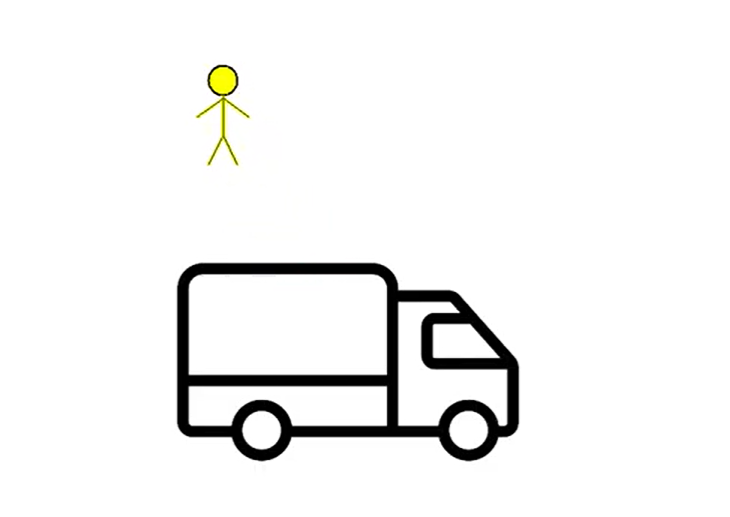
\includegraphics[width=0.8\linewidth]{images/Stickman Gelb.png}\\[1ex]
    \centering
    \caption{Gelb - Warnung, Gefahr möglich}
    \label{ABBILDUNG}
\end{figure}
\begin{figure}[H]
    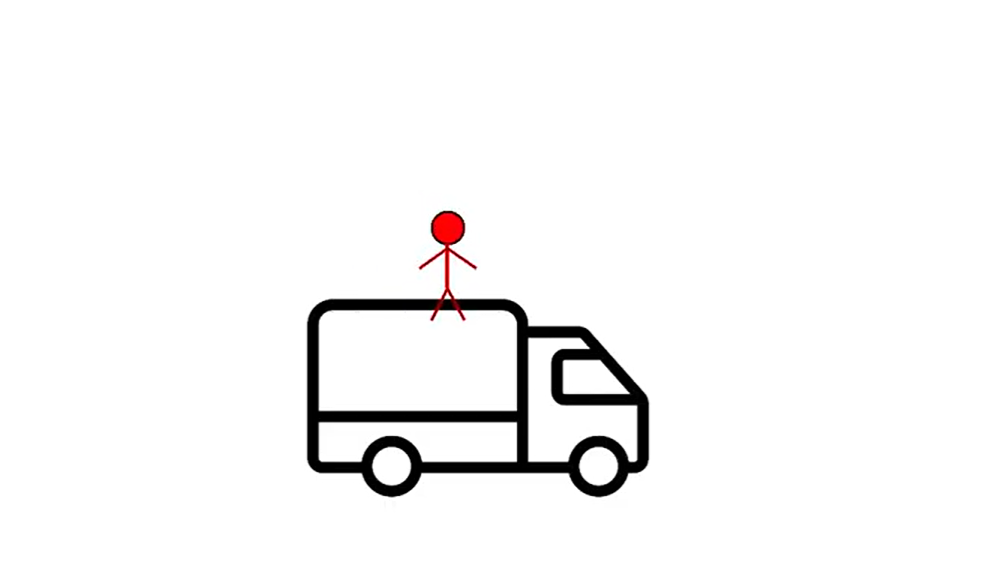
\includegraphics[width=1\linewidth]{images/Stickman Rot.png}\\[1ex]
    \centering
    \caption{Rot - Achtung, Kollisionsgefahr}
    \label{ABBILDUNG}
\end{figure}

\paragraph{Visualisierung der Antennen und Sensorlinien}

Die Position der Antennenarrays wird grafisch dargestellt und durch Linien ergänzt, welche die gemessenen Einfallswinkel (\ac{AoA}) andeuten. Diese Linien 
zeigen die theoretische Messrichtung, was ein besseres Verständnis der Triangulation erlaubt.

\begin{figure}[H]
    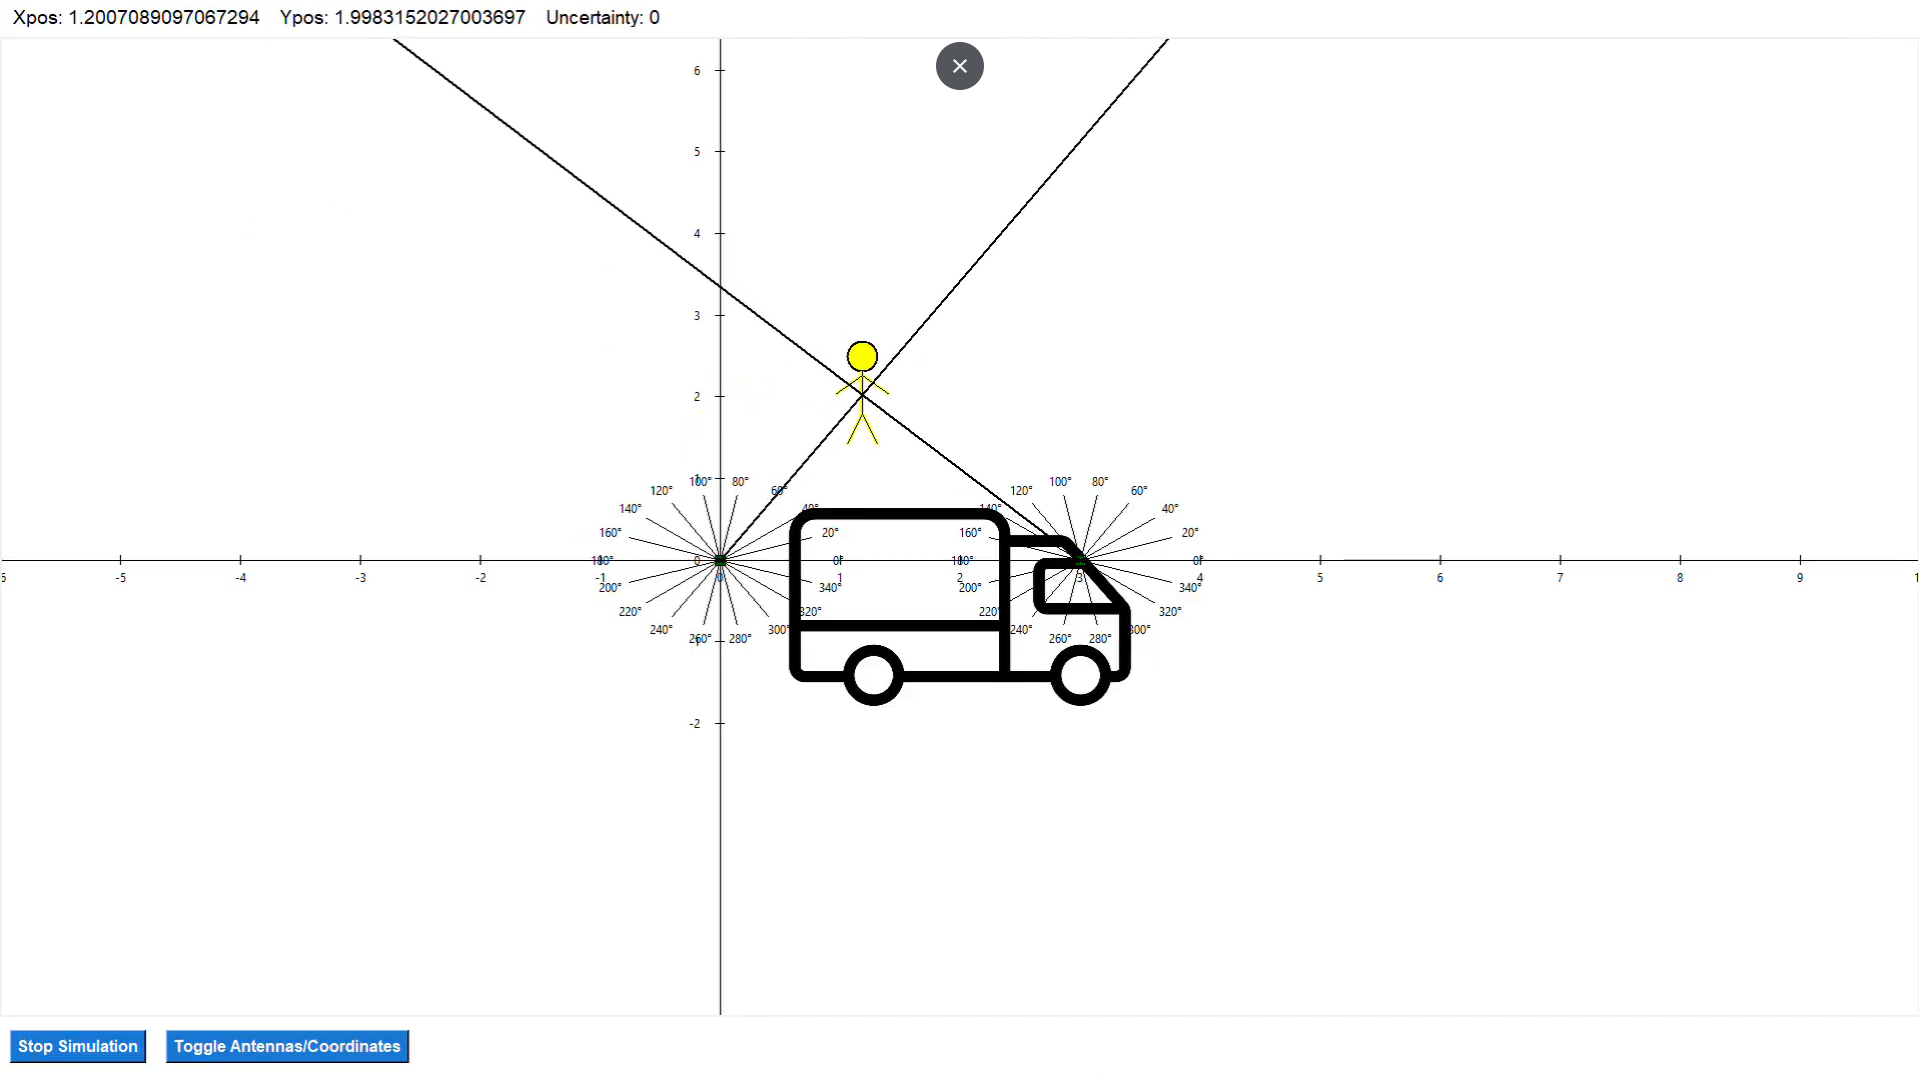
\includegraphics[width=1\linewidth]{images/Visualisierung Antennen.png}\\[1ex]
    \centering
    \caption{Visualisierung der Antennen und Sensorlinien}
    \label{ABBILDUNG}
\end{figure}

\paragraph{Interaktive Steuerung und Optimierungen}

Ein zentrales Element ist die Möglichkeit, zwischen verschiedenen Visualisierungsmodi umzuschalten. Über ein Toggle-Button kann die Darstellung der 
Koordinatenachsen und Sensorlinien aktiviert oder ausgeblendet werden, um je nach Anwendungsfall zwischen technischer Analyse und Präsentation zu 
wechseln. Zusätzlich kann die Darstellung bei Bedarf in den Vollbildmodus gesetzt werden.

Zur Steuerung und flexiblen Nutzung wurde außerdem eine ausführbare Batch-Datei (\texttt{.bat}) bereitgestellt, mit der definierte Logdateien gezielt 
abgespielt und getestet werden können. Diese Struktur erlaubt es, mehrere gespeicherte Datensätze individuell zu benennen, abzurufen und ohne 
Hardwarebezug zu analysieren.

\begin{figure}[H]
    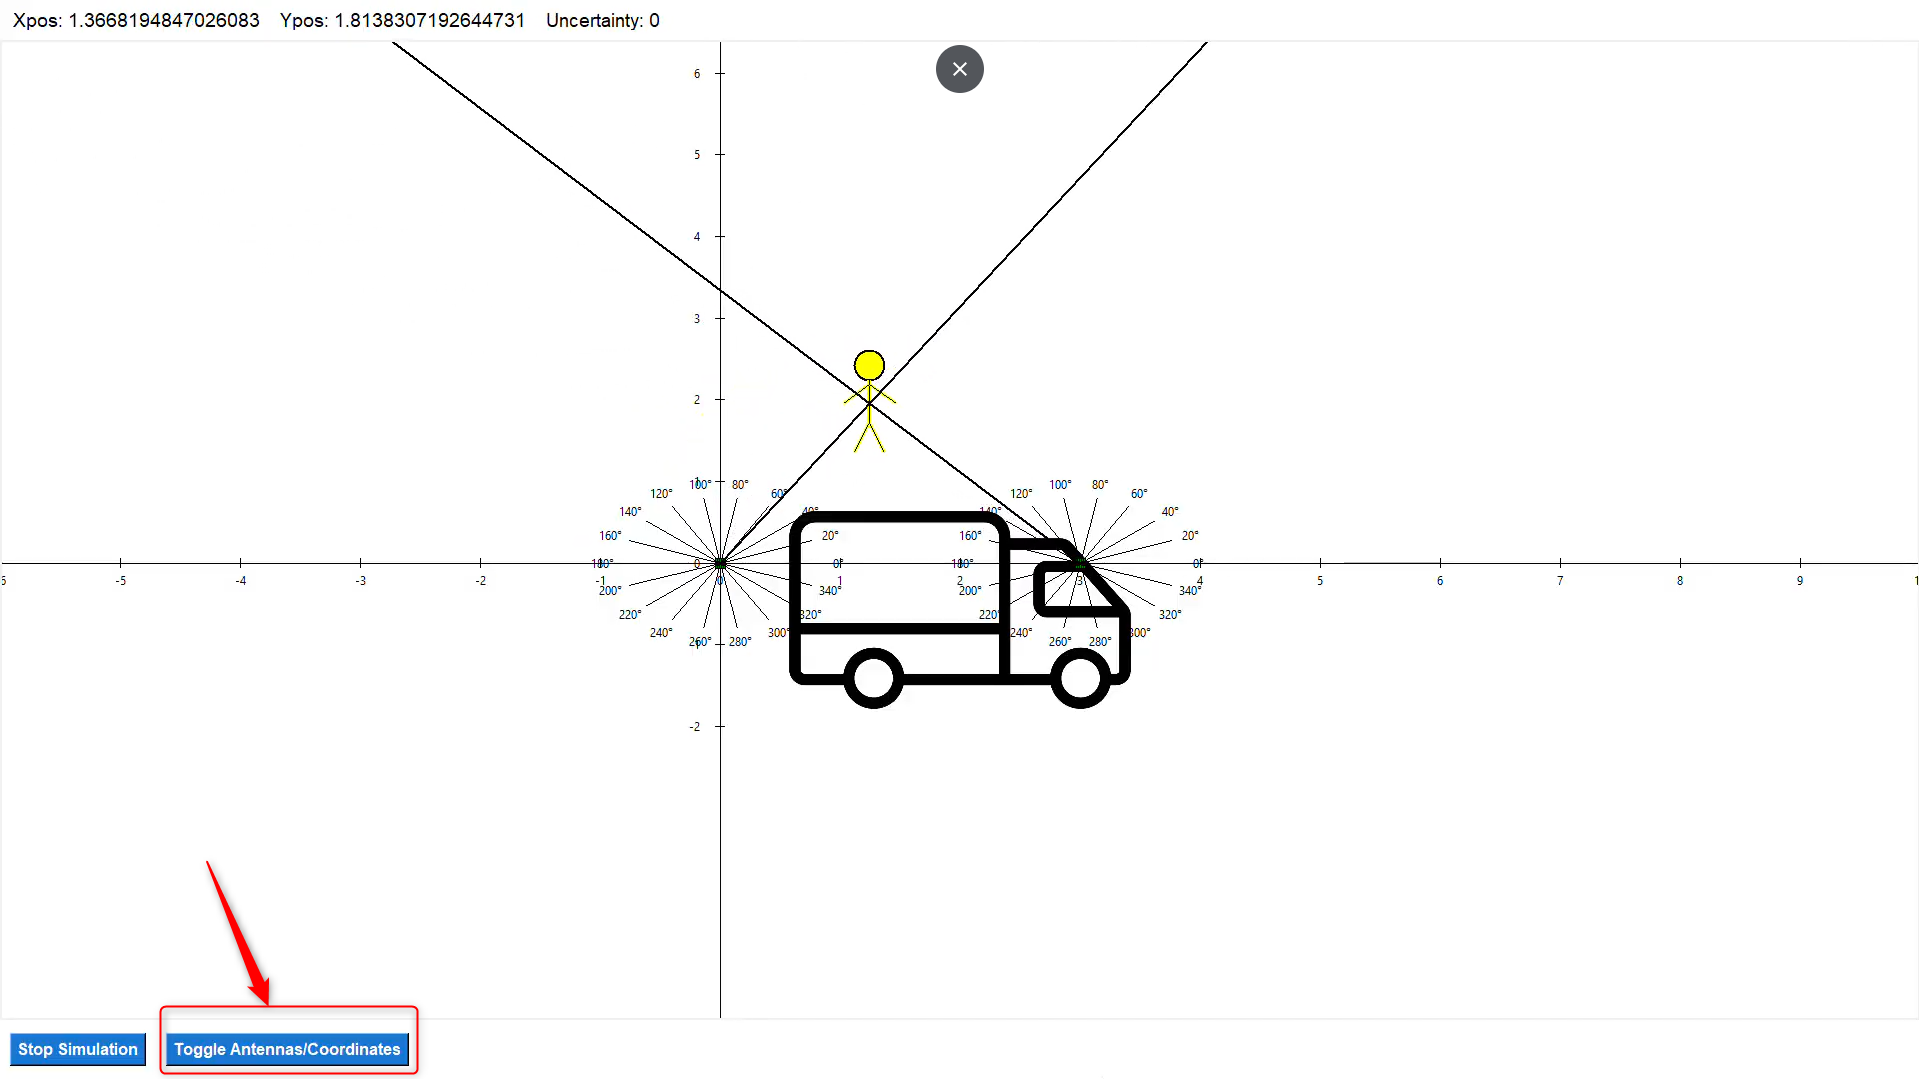
\includegraphics[width=1\linewidth]{images/Volle Darstellung.png}\\[1ex]
    \centering
    \caption{Volle Darstellung Benutzeroberfläche}
    \label{ABBILDUNG}
\end{figure}
\begin{figure}[H]
    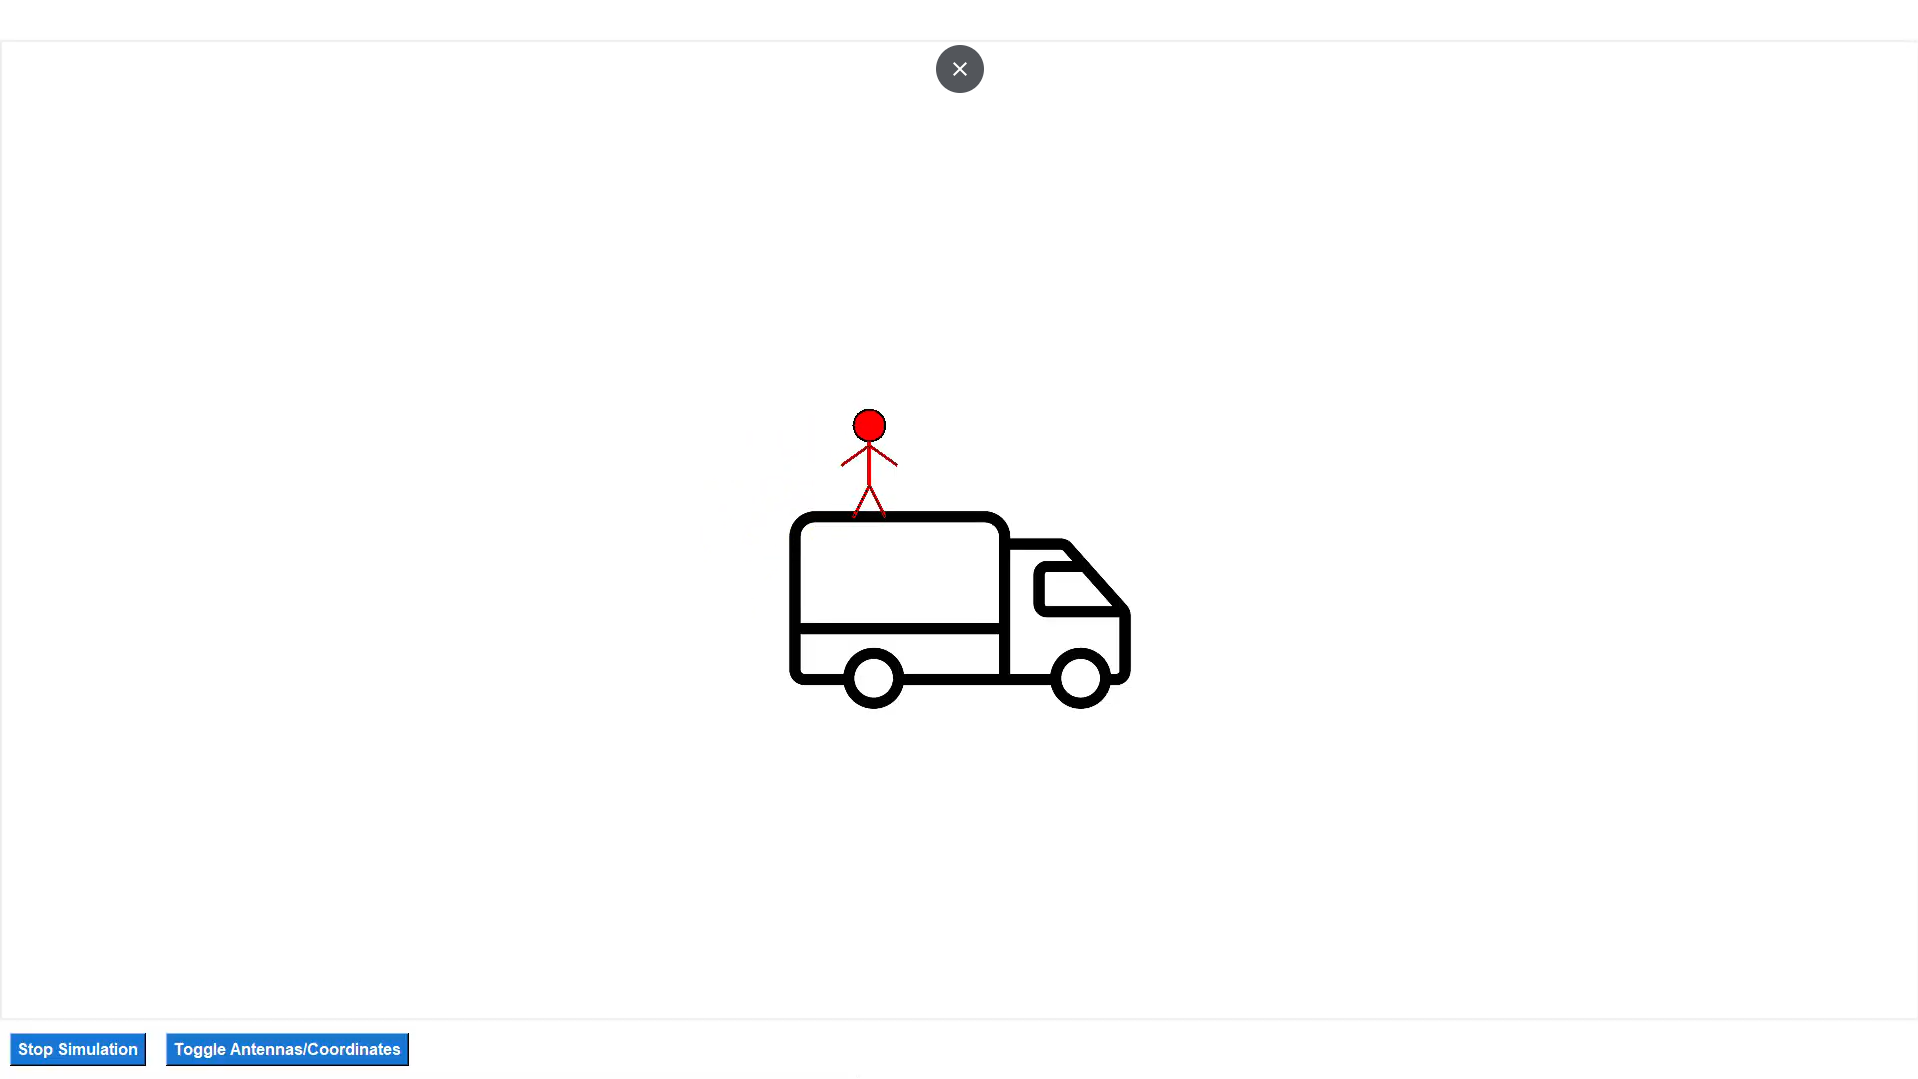
\includegraphics[width=1\linewidth]{images/Minimale Darstellung.png}\\[1ex]
    \centering
    \caption{Minimale Darstellung Benutzeroberfläche}
    \label{ABBILDUNG}
\end{figure}

\paragraph{Zusammenfassung}

Die überarbeitete Visualisierung stellt eine signifikante Verbesserung gegenüber der früheren Version dar. Sie bietet nicht nur eine realitätsnähere 
und dynamischere Darstellung der Position des Tags, sondern erleichtert durch optionale Darstellungselemente und glattere Bewegung auch die Analyse und 
Präsentation für unterschiedliche Zielgruppen. Gleichzeitig wurde Wert auf eine modulare und wartbare Struktur gelegt, sodass zukünftige 
Erweiterungen – etwa die Integration weiterer Visualisierungselemente oder zusätzlicher Sensoren – problemlos möglich sind.

\subsection{Ergebnisse und Benutzerfreundlichkeit}

Die Implementierung der verbesserten Visualisierung zeigt insgesamt funktionale Fortschritte und eine gesteigerte Benutzerfreundlichkeit. Die Anbindung 
über \ac{TCP} funktioniert stabil sowohl im Echtzeitbetrieb mit Live-Messdaten als auch im Offline-Modus über den Datenlogger. Dies ermöglicht eine flexible 
Analyse und Bewertung von Positionsdaten ohne permanenten Zugriff auf die Hardware. Die Integration der Replay-Funktion in die Benutzeroberfläche verläuft
nahtlos – gespeicherte Daten werden zuverlässig geladen, verarbeitet und dargestellt. Dies bietet insbesondere im Entwicklungs- und Testkontext deutliche
Vorteile, da Anpassungen und neue Algorithmen unabhängig von einer aktiven Messumgebung evaluiert werden können.

Im Bereich der Darstellung konnte mit der Ersetzung des bisherigen Tag-Punktes durch eine abstrahierte Stickman-Figur ein deutlicher visueller 
Fortschritt erzielt werden. Zusätzlich wurden Warnstufen eingeführt, welche die Distanz zu einem virtuellen \ac{LKW} durch Farbwechsel (grün, gelb, rot) 
kodieren. Auch die Antennenpositionen und deren Richtungsinformation werden grafisch dargestellt, wenngleich deren Schnittpunkt noch nicht exakt mit der 
berechneten Tag-Position übereinstimmt. Insgesamt ist die Visualisierung deutlich intuitiver und eignet sich besser zur Präsentation auf Fachmessen oder
vor nicht-technischem Publikum. Ein optional zuschaltbares Koordinatensystem erlaubt zudem eine differenzierte technische Auswertung.

Die Bewegung des Tags erscheint derzeit noch leicht ruckartig und verzögert. Es wurden bereits Maßnahmen zur Glättung durch exponentielles Smoothing 
implementiert, allerdings zeigen sich in der Praxis weiterhin Limitierungen, die in zukünftigen Iterationen adressiert werden müssen.

Die Bedienbarkeit der Oberfläche ist insgesamt positiv zu bewerten. Die grafische Benutzeroberfläche zeigt beim Start die relevanten Schaltflächen gut 
sichtbar an. Durch den Toggle-Modus können Darstellungsmodi flexibel gewechselt werden – beispielsweise die Ein- und Ausblendung technischer Hilfslinien. 
Die Benutzerführung ist intuitiv und ermöglicht auch technisch weniger versierten Anwendern eine effiziente Nutzung.

Zusammenfassend lässt sich festhalten, dass die entwickelte Benutzeroberfläche eine stabile Basis für zukünftige Erweiterungen bietet. Neue Features 
können mit überschaubarem Aufwand ergänzt werden, und die vorhandene Architektur erlaubt eine Trennung von Datenaufnahme und Visualisierung. Damit stellt
das System ein praktikables Werkzeug für die Weiterentwicklung, Testung und Demonstration von Assistenzsystemen dar.

\section{Test und Validierung}
\subsection{Testmethodik und -umgebung}

Ziel der Tests war es, die Funktionsweise der entwickelten Komponenten -- insbesondere des Datenloggers und der neuen Visualisierung -- in einer 
realitätsnahen, aber bewusst reduzierten Umgebung zu validieren. Es handelte sich dabei nicht um umfangreiche Praxistests in verschiedensten 
Anwendungsszenarien, sondern um gezielte Funktionstests, die Fehlerquellen aufdecken und Verbesserungspotenziale aufzeigen sollten \cite{myers_testing}.

\paragraph{Testziele}
Im Mittelpunkt stand die Überprüfung folgender Aspekte:
\begin{itemize}
    \item Funktion der Datenerfassung, Speicherung und Wiedergabe im Replay-Modus
    \item Konsistenz der \ac{TCP}-Kommunikation zwischen Logger und \ac{UI}
    \item korrekte Verarbeitung gespeicherter \ac{JSONL}-Daten \cite{json_processing_books}
    \item visuelle Rückmeldung in der Benutzeroberfläche (z.\,B. Darstellung des Tags, Antennen und Warnfarben)
    \item allgemeine Bedienbarkeit und Reaktion der UI-Komponenten \cite{nielsen_usability}
\end{itemize}

\paragraph{Testarten}
Es wurden verschiedene Testarten angewandt:
\begin{itemize}
    \item \textbf{Funktionstests}: Einzelne Module wurden separat geprüft (z.\,B. Speicherung, Wiedergabe, Visualisierung)
    \item \textbf{Integrationstests}: Zusammenspiel von Datenlogger, Netzwerkverbindung und Visualisierung
    \item \textbf{Systemtests}: Gesamtprüfung mit Live- oder gespeicherten Datenströmen
\end{itemize}

\paragraph{Testumgebung}
Die Tests wurden auf einem Standard-PC unter Windows 11 mit Python 3.12 durchgeführt. Die Kommunikation lief lokal über eine \ac{TCP}-Verbindung 
(\texttt{localhost}), was eine stabile Übertragung ohne externe Netzwerkeinflüsse sicherstellte. Als Datenbasis kamen sowohl Live-Messungen mit 
angeschlossener Hardware als auch gespeicherte \ac{JSONL}-Dateien aus früheren Sessions zum Einsatz. Die grafische Benutzeroberfläche wurde dabei im 
Vollbildmodus auf einem 17-Zoll-Bildschirm (Laptop) betrieben.

\paragraph{Ablauf}
Die Tests erfolgten manuell. Zunächst wurde die Verbindung zwischen Logger und UI geprüft. Anschließend wurden verschiedene Datensätze -- sowohl reale
Messungen als auch synthetische Beispiele -- über die \texttt{replayLogger.py} wiedergegeben. Dabei wurde beobachtet, wie die \ac{UI} auf Positionsdaten, 
Sensordaten und Änderungen in der Darstellung reagiert. Auch die neue Funktion zur Darstellung eines Stickmans und des \ac{LKW}-Bildes wurde systematisch 
getestet. Der Wechsel des Darstellungsmodus (z.\,B. Ein-/Ausblenden der Achsen) wurde ebenfalls geprüft.

Ergänzend dazu wurde gezielt versucht, typische Grenzsituationen und Extremszenarien zu simulieren. Dazu gehörten beispielsweise sehr schnelle oder 
sehr langsame Bewegungen des Tags sowie Positionen am äußersten linken oder rechten Rand des Koordinatensystems. Ziel war es zu prüfen, ob die 
Positionsberechnung, Visualisierung und Stabilität auch in diesen Randbereichen erwartungsgemäß funktionieren.

\paragraph{Einschränkungen}
Aufgrund zeitlicher und infrastruktureller Begrenzungen wurde auf umfangreiche Feldversuche oder Szenarien im Realbetrieb verzichtet. Ziel 
war primär eine funktionale Prüfung der neu entwickelten Komponenten. Eine tiefgreifende Evaluierung im produktiven Umfeld ist für spätere 
Projektphasen vorgesehen.

\subsection{Ergebnisse der Tests}

Die durchgeführten Tests hatten zum Ziel, die grundsätzliche Funktionalität des entwickelten Datenloggers sowie der erweiterten Visualisierung zu 
überprüfen. Dabei standen insbesondere Aspekte wie Datenintegrität, Kommunikation, Benutzerfreundlichkeit und visuelle Darstellung im Vordergrund.

\paragraph{Funktionalität und Kommunikation}
Die Tests zeigten, dass die Speicherung der erfassten Sensordaten im \ac{JSONL}-Format zuverlässig funktioniert. Auch die Wiedergabe der gespeicherten Daten 
im Replay-Modus über \texttt{replayLogger.py} erwies sich als stabil. Die \ac{TCP}-Kommunikation zwischen Datenlogger und grafischer Benutzeroberfläche konnte 
ohne Verbindungsabbrüche oder Datenverluste durchgeführt werden. Es war möglich, sowohl reale Messdaten als auch gespeicherte Daten aus dem Logger 
erfolgreich in die Benutzeroberfläche zu laden.

\paragraph{Darstellung des Tags}
Die Bewegung des Tags innerhalb der grafischen Oberfläche erwies sich noch als verbesserungsbedürftig. Obwohl bereits ein Glättungsalgorithmus 
implementiert wurde, wirkt die Bewegung weiterhin leicht verzögert und ruckartig. Besonders bei Extrempositionen – also wenn sich der Tag weit 
rechts oder links außerhalb des zentralen Bereichs bewegt – konnte beobachtet werden, dass die Ortung deutlich an Genauigkeit verliert. Dies liegt
am zugrunde liegenden Triangulationsverfahren: Wenn sich beide gemessenen Winkel stark überlagern, ist eine exakte Positionsbestimmung kaum noch 
möglich \cite{triangulation_geometry}.

\begin{figure}[H]
    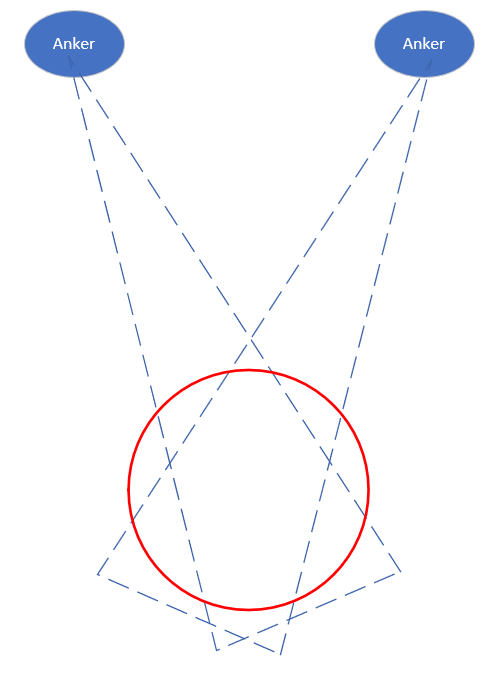
\includegraphics[width=0.5\linewidth]{images/Gute Triangulation.png}\\[1ex]
    \centering
    \caption{Gute Triangulation}
    \label{ABBILDUNG}
\end{figure}
\begin{figure}[H]
    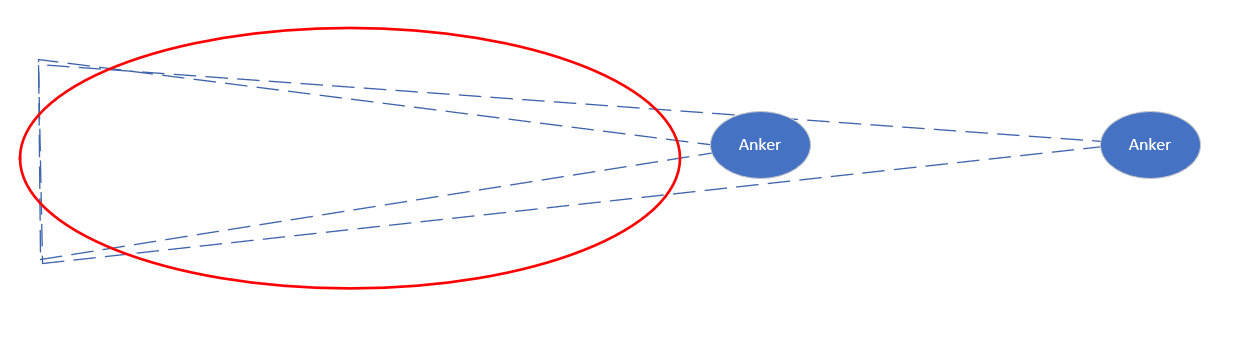
\includegraphics[width=1\linewidth]{images/Schlechte Triangulation.png}\\[1ex]
    \centering
    \caption{Schlechte Triangulation}
    \label{ABBILDUNG}
\end{figure}

\paragraph{Visualisierung und Layout}
Die Darstellung wurde im Vergleich zum vorherigen Zustand deutlich verbessert. Anstelle eines einfachen Punktes wird der Tag nun als stilisierter 
Stickman visualisiert. Darüber hinaus wurde ein \ac{LKW}-Bild zur Verdeutlichung der Anwendungssituation ergänzt. Die Antennenpositionen werden 
grafisch dargestellt und mit Richtungslinien versehen, welche sich in den meisten Fällen korrekt im Bereich der ermittelten Position schneiden – ein 
klares visuelles Feedback über die Funktionsweise des Systems. Dennoch bleibt die Darstellung grundsätzlich einfach gehalten. Zusätzliche 
Visualisierungselemente wie eine Geschwindigkeitsanzeige, eine dynamische Skalierung des Bewegungsraums oder realistischere Proportionen der 
dargestellten Objekte könnten künftig integriert werden.

\paragraph{Benutzerfreundlichkeit}
Die Benutzeroberfläche erwies sich in der Praxis als einfach zu bedienen. Beim Starten des Programms werden klar beschriftete Schaltflächen angezeigt, 
die ohne Vorkenntnisse verständlich sind. Funktionen wie das Starten und Stoppen der Simulation oder das Umschalten von Koordinaten- und Antennenanzeige 
sind intuitiv zugänglich. Die Implementierung der \ac{BAT}-Datei zum Start des Datenloggers erleichtert zusätzlich die Bedienung, insbesondere für unerfahrene
Nutzer \cite{nielsen_usability}. Zudem kann zwischen verschiedenen gespeicherten Messreihen gewählt, diese umbenannt und erneut abgespielt werden.

\paragraph{Zusammenfassende Bewertung}
Insgesamt wurde mit dem entwickelten System ein funktionaler Prototyp geschaffen, der die gewünschten Kernfunktionen erfüllt. Die Integration des 
Datenloggers in die bestehende Softwareumgebung ist gelungen und erlaubt eine flexible Nutzung, sowohl online als auch offline. Die Visualisierung 
ist verständlicher als zuvor, besonders im Hinblick auf Präsentationen und Messen. Dennoch bestehen in mehreren Bereichen Potenziale zur weiteren 
Optimierung, insbesondere in der flüssigen Bewegung des Tags, in der Genauigkeit der Darstellung sowie in der Erweiterung des visuellen Feedbacks für
komplexere Anwendungsszenarien.

\subsection{Diskussion der Testergebnisse und Optimierungspotentiale}

Die durchgeführten Funktionstests zeigen, dass die wesentlichen Kernziele – insbesondere die prototypische Realisierung des Datenloggers und 
dessen Anbindung an die Visualisierung – erfüllt wurden. Dennoch offenbaren die Testergebnisse mehrere Schwachstellen und Hinweise auf künftigen 
Verbesserungsbedarf, die im Folgenden diskutiert werden.

\paragraph{Limitierungen in der Positionsdarstellung}

Trotz implementierter Glättungsmechanismen bleibt die Bewegung des Tags auf der Benutzeroberfläche merklich ruckartig. Insbesondere bei 
schnellen Richtungswechseln oder Bewegungen am Rand des Koordinatensystems treten Verzögerungen auf. Dies kann auf die gewählten Smoothing-Parameter 
oder das einfache Exponentialfilter-Verfahren zurückgeführt werden \cite{signal_filtering}, das bei dynamischen Bewegungen an seine Grenzen stößt. Eine adaptive Glättung, die 
sich an der Bewegungsgeschwindigkeit orientiert, könnte hier künftig Abhilfe schaffen.

Ein weiterer kritischer Punkt ist die eingeschränkte Genauigkeit der Positionsbestimmung bei extremen Positionen. Wenn sich der Tag sehr weit 
links oder rechts außerhalb der Hauptmessachse befindet, versagt die Triangulation teilweise. Der Grund liegt in der Geometrie der \ac{AoA}-Messung: 
Bei annähernd parallelen Winkelmessungen zweier Anker wird der Schnittpunkt der Geraden numerisch instabil, was eine präzise Lokalisierung erschwert \cite{triangulation_geometry}.

\paragraph{Darstellung und Interpretation der Ergebnisse}

Die Visualisierung wurde gegenüber der ursprünglichen Version deutlich verbessert. Die Einführung eines symbolischen Stickman-Modells sowie 
eines schematischen \ac{LKW}-Bildes erhöht die Verständlichkeit, besonders für externe Zielgruppen oder Präsentationen. Gleichzeitig bleibt die 
grafische Ausgestaltung noch rudimentär. Elemente wie Maßstabsanzeige, Bewegungsverläufe, Risikozonen oder Geschwindigkeitspfeile fehlen bislang, 
könnten aber die Interpretation der Szenarien erheblich erleichtern.

Darüber hinaus könnte auch die Proportionalität zwischen realer Bewegung und Koordinatensystem verbessert werden. Aktuell ist die Zuordnung zwischen 
physischer Verschiebung und grafischer Darstellung nicht intuitiv nachvollziehbar, was insbesondere bei der Validierung der Messergebnisse hinderlich 
sein kann.

\paragraph{Bedienbarkeit und Nutzbarkeit}

Die Bedienung der Visualisierungsoberfläche gestaltet sich insgesamt benutzerfreundlich. Die eingefügten Steuerungselemente (z.\,B. Toggle-Schalter 
für die Darstellung der Koordinatenachsen) sowie die Möglichkeit, das Programm per \texttt{.bat}-Datei zu starten, erleichtern die Nutzung auch für 
weniger erfahrene Anwender. Die einfache Darstellung ist für erste Tests und Demonstrationen durchaus ausreichend, lässt sich jedoch hinsichtlich 
Detailtiefe und Flexibilität weiterentwickeln.

\paragraph{Potenziale zur Erweiterung}

Für die Weiterentwicklung ergeben sich mehrere sinnvolle Ansätze. Neben einer grafischen Verfeinerung könnten folgende Maßnahmen zur 
Optimierung beitragen:

\begin{itemize}
    \item Einführung eines dynamischen Zoom- oder Perspektivmodus zur besseren Verfolgung der Tag-Bewegung
    \item Erweiterung der Darstellung um Geschwindigkeit, Bewegungsrichtung und Unsicherheitsbereiche
    \item Modularisierung der Visualisierung zur einfacheren Einbindung weiterer Objekte oder Assistenzsysteme
    \item Verbesserung der Glättungslogik mit adaptiven oder maschinellen Verfahren
    \item Vorbereitung auf künftige Erweiterungen wie eine 3D-Ansicht oder AR-Darstellung
\end{itemize}

\paragraph{Fazit}

Die bisherigen Testergebnisse zeigen eine solide Basis, auf der sich weiter aufbauen lässt. Sowohl die technische Funktionalität als auch die visuelle
Vermittlung der Daten sind grundsätzlich gegeben, müssen jedoch für eine belastbare Systembewertung und breitere Nutzbarkeit noch weiterentwickelt und 
verfeinert werden.

\section{Kritische Bewertung und Ausblick}
\subsection{Reflexion der erreichten Ergebnisse}

Im Rahmen dieser Arbeit wurde das Ziel verfolgt, ein robustes Datenloggersystem zu entwickeln sowie die bestehende Visualisierung einer 
Bluetooth-\ac{AoA}-basierten Lokalisierungslösung gezielt zu erweitern. Rückblickend lässt sich feststellen, dass wesentliche Kernziele erfolgreich 
umgesetzt wurden.

Der entwickelte Datenlogger ermöglicht eine strukturierte und flexible Erfassung sowie Speicherung von Messdaten im \ac{JSONL}-Format. Er erlaubt eine 
spätere Wiedergabe der Daten ohne Hardwareeinsatz und schafft somit eine effektive Grundlage für Tests, Parametrierung und Algorithmenentwicklung. 
Die Integration des Loggers in die bestehende Softwareumgebung erfolgte reibungslos durch ein separates Python-Skript mit minimalen Änderungen am 
Ursprungscode. Auch die Konnektivität zur Benutzeroberfläche über eine \ac{TCP}-Verbindung funktionierte stabil, sowohl im Live-Betrieb als auch im 
Replay-Modus.

Auf Seiten der Visualisierung wurde die bisher sehr reduzierte Darstellung um mehrere Elemente erweitert. Die Verwendung eines stilisierten 
Stickman-Modells zur Repräsentation des Tags, die Einbindung eines realitätsnahen \ac{LKW}-Bildes sowie die farbliche Warnstufendarstellung 
führten zu einer deutlich verständlicheren und praxistauglicheren Repräsentation. Dies ist insbesondere im Hinblick auf externe Präsentationen, 
z.\,B. auf Messen oder in interdisziplinären Gremien, ein entscheidender Vorteil.

Trotz dieser Fortschritte zeigen sich auch einige Grenzen. Die Bewegung des Tags ist nach wie vor leicht verzögert und nicht vollständig flüssig, 
obwohl bereits erste Maßnahmen zur Glättung implementiert wurden. In Randbereichen des Messfeldes stößt die Triangulation durch sich überlappende 
Winkelpaare an ihre mathematischen Grenzen, was zu ungenauen oder nicht vorhandenen Positionsschätzungen führt. Auch die visuelle Darstellung – etwa in 
Bezug auf Maßstäblichkeit oder ergänzende Informationen wie Geschwindigkeit – bietet weiteres Verbesserungspotenzial.

Nichtsdestotrotz konnte durch die modulare Struktur, den Einsatz etablierter Technologien (Python, JSON, \ac{TCP}) sowie den pragmatischen Ansatz ein 
funktionierendes System geschaffen werden, das die Grundlage für weiterführende Entwicklungen bietet. Die Arbeit zeigt damit deutlich, dass durch 
gezielte Ergänzungen und strukturiertes Vorgehen auch in einer begrenzten Projektlaufzeit signifikante Fortschritte in Funktionalität und 
Benutzerfreundlichkeit erzielt werden können.

\subsection{Grenzen der aktuellen Umsetzung}

Trotz der erfolgreichen Umsetzung eines funktionalen Datenloggers und einer verbesserten Visualisierung bestehen derzeit noch mehrere Einschränkungen, 
die das System in seiner Einsatzbreite und Qualität begrenzen.

\paragraph{Begrenzte Genauigkeit der Positionsbestimmung} 
Die Positionsschätzung des Tags basiert auf Triangulation aus den gemessenen \ac{AoA}-Winkeln zweier Anker. Dieses Verfahren liefert nur dann 
zuverlässige Ergebnisse, wenn die geometrische Anordnung der Anker günstig gewählt ist. Besonders bei Messungen an den Rändern des definierten 
Messfelds (z.\,B. weit links oder rechts) kann es aufgrund der Überlagerung oder Parallelität der Winkellinien zu ungenauen oder gar nicht 
berechenbaren Positionen kommen.

\paragraph{Nicht vollständig realitätsgetreue Bewegungsdarstellung}
Obwohl Maßnahmen zur Glättung der Bewegung (z.\,B. mittels Pufferung und Smoothing) umgesetzt wurden, wirkt die Visualisierung des bewegten 
Tags weiterhin leicht ruckartig und reagiert nicht in Echtzeit. Zudem fehlt derzeit eine maßstabsgetreue Übertragung der tatsächlichen Bewegung 
auf die Bildschirmanzeige.

\paragraph{Einfaches visuelles Layout}
Die Visualisierung nutzt bisher einfache grafische Elemente wie einen stilisierten Stickman und ein eingefügtes Bild eines \ac{LKW}s. 
Die Darstellung unterstützt die Verständlichkeit, lässt jedoch hinsichtlich Detailtiefe, Ästhetik und Interaktivität noch deutlichen Spielraum 
für Verbesserungen. Eine Möglichkeit zur perspektivischen Darstellung, Animation komplexerer Objekte oder eine interaktive Benutzersteuerung ist 
bislang nicht vorgesehen.

\paragraph{Begrenzte Testtiefe}
Die entwickelte Lösung wurde im Rahmen kleinerer Testszenarien mit kurzer Laufzeit erprobt. Umfangreiche Testreihen unter realitätsnahen 
Bedingungen – etwa mit komplexer Bewegung, Störeinflüssen oder Mehrpersonen-Szenarien – konnten zeitbedingt nicht durchgeführt werden.

\paragraph{Fehlende erweiterte Analyse- und Mehrbenutzerfunktionen}
Die aktuelle Implementierung erlaubt eine visuelle Einzelnutzung mit Echtzeitdarstellung bzw. Offline-Replay. Weiterführende Funktionalitäten wie 
gleichzeitiger Mehrbenutzerzugriff, interaktive Analysewerkzeuge, Exportfunktionen oder statistische Auswertungen (z.\,B. Heatmaps) sind derzeit nicht 
enthalten.

\paragraph{Technische Einschränkungen der Visualisierung}
Die Umsetzung der Benutzeroberfläche auf Basis von Python und Tkinter bringt den Vorteil einer schnellen Realisierbarkeit, schränkt jedoch die 
grafischen und performanten Möglichkeiten ein. Zudem erfordert der Datenlogger eine strukturierte Ablage der \ac{JSONL}-Dateien und Pfade, was die 
Portabilität des Systems derzeit noch begrenzt.

Diese Punkte zeigen klar auf, in welchen Bereichen gezielte Weiterentwicklungen erforderlich sind, um das System robuster, skalierbarer und 
praxistauglicher zu gestalten.

\subsection{Vorschläge für zukünftige Weiterentwicklungen}

Basierend auf den Ergebnissen und Erkenntnissen der bisherigen Arbeit ergeben sich verschiedene Ansatzpunkte für eine sinnvolle Weiterentwicklung
des entwickelten Systems.

\paragraph{Technische Optimierung der Bewegungsglättung}
Die Bewegung des Tags ist in der aktuellen Visualisierung noch nicht ausreichend flüssig. Obwohl bereits ein Kalman-basiertes Glättungsverfahren 
implementiert wurde, treten weiterhin ruckartige Darstellungen und spürbare Verzögerungen auf. Eine Verbesserung kann erzielt werden, indem die 
Kalman-Parameter – etwa Prozess- und Messrauschen – adaptiv angepasst und feiner auf die Dynamik des Systems abgestimmt werden, um eine realitätsnähere
 Bewegung des Tags zu erreichen \cite{kalman_filter_book}.

\paragraph{Verbesserung der Triangulation bei Randlagen}
Ein beobachtetes Problem betrifft die Genauigkeit der Positionsbestimmung, insbesondere wenn sich das Tag am Rand des Erfassungsbereichs befindet. 
Hierbei treten geometrische Probleme auf, da die beiden Winkelmessstrahlen nahezu parallel verlaufen und die Schnittpunktbestimmung ungenau wird. 
Eine Möglichkeit zur Verbesserung besteht in der Integration eines dritten Antennen-Boards. Durch die zusätzliche Winkelmessung kann die geometrische 
Ambiguität reduziert und die Lokalisierungsgenauigkeit signifikant gesteigert werden.

\paragraph{Erweiterung der Replay-Funktionalität}
Der Datenlogger erlaubt bereits das Abspielen aufgezeichneter Messdaten. In zukünftigen Versionen könnte diese Funktion erweitert werden, um Parameter 
direkt über eine grafische Benutzeroberfläche anpassen zu können. Eine visuelle Konfigurationsmaske mit Live-Feedback würde die Entwicklungs- und 
Testphase erheblich vereinfachen.

\paragraph{Erweiterung der Visualisierungsmöglichkeiten}
Die Visualisierung des Tags wurde bereits durch einen stilisierten Stickman sowie ein \ac{LKW}-Modell ergänzt. Um jedoch noch realitätsnähere und
professionellere Darstellungen zu ermöglichen – insbesondere bei öffentlichen Vorführungen oder Messen – könnten 3D-Modelle eingesetzt werden. 
Auch zusätzliche visuelle Indikatoren wie Bewegungstrails, Heatmaps oder Geschwindigkeitssymbole wären denkbar \cite{unity_visualization}.

Zudem könnte das Koordinatensystem um interaktive Funktionen wie Zoom, Skalierung oder Ein-/Ausblendung erweitert werden. Mittelfristig wäre auch 
der Umstieg auf eine leistungsfähigere Visualisierungsplattform, etwa auf Basis von Unity3D oder WebGL, zu evaluieren \cite{webgl_book}.

\paragraph{Verbesserung der Benutzeroberfläche}
Die aktuelle \ac{UI} bietet bereits eine grundlegend benutzerfreundliche Bedienung. Zukünftig wäre jedoch eine webbasierte Variante wünschenswert, 
die plattformunabhängig funktioniert und auch über mobile Endgeräte steuerbar ist. Eine intuitive Konfiguration von Replay-, Logging- und 
Visualisierungsparametern würde die Nutzerfreundlichkeit zusätzlich steigern \cite{ux_design_book}.

\paragraph{Tests und Validierung}
Die durchgeführten Tests waren in ihrem Umfang noch begrenzt. Für zukünftige Weiterentwicklungen sollte ein strukturierter Testkatalog 
entwickelt werden, der typische Anwendungsszenarien, Grenzfälle und Langzeittests umfasst. Dadurch ließe sich die Robustheit und Zuverlässigkeit 
der Lösung weiter erhöhen.

\paragraph{Systemintegration und Modularisierung}
Langfristig wäre eine stärkere Modularisierung der Softwarestruktur anzustreben. Durch eine saubere Trennung von Datenaufnahme, Auswertung, 
Visualisierung und Replay-Modulen ließe sich die Wartbarkeit verbessern. Auch die Integration externer Sensoren oder Cloud-Plattformen zur 
weitergehenden Analyse könnte über standardisierte Schnittstellen ermöglicht werden \cite{software_architecture_modular}.

\paragraph{Zusammenfassung}
Insgesamt existieren vielfältige Ansatzpunkte für die Weiterentwicklung der Lösung. Diese reichen von technischen Verbesserungen der 
Positionsbestimmung und Visualisierung über benutzerfreundliche \ac{UI}-Konzepte bis hin zur Erweiterung des Hardware-Setups durch zusätzliche Anker. 
Gerade die Kombination dieser Maßnahmen verspricht eine deutliche Steigerung der Systemqualität und Anwendbarkeit in praxisnahen Einsatzszenarien.

%---------------------------------------------------------
% Bibliografie
%---------------------------------------------------------
\begingroup
\sloppy
\nocite{*}
\printbibliography

\end{document}
